\PassOptionsToPackage{unicode=true}{hyperref} % options for packages loaded elsewhere
\PassOptionsToPackage{hyphens}{url}
%
\documentclass[]{book}
\usepackage{lmodern}
\usepackage{amssymb,amsmath}
\usepackage{ifxetex,ifluatex}
\usepackage{fixltx2e} % provides \textsubscript
\ifnum 0\ifxetex 1\fi\ifluatex 1\fi=0 % if pdftex
  \usepackage[T1]{fontenc}
  \usepackage[utf8]{inputenc}
  \usepackage{textcomp} % provides euro and other symbols
\else % if luatex or xelatex
  \usepackage{unicode-math}
  \defaultfontfeatures{Ligatures=TeX,Scale=MatchLowercase}
\fi
% use upquote if available, for straight quotes in verbatim environments
\IfFileExists{upquote.sty}{\usepackage{upquote}}{}
% use microtype if available
\IfFileExists{microtype.sty}{%
\usepackage[]{microtype}
\UseMicrotypeSet[protrusion]{basicmath} % disable protrusion for tt fonts
}{}
\IfFileExists{parskip.sty}{%
\usepackage{parskip}
}{% else
\setlength{\parindent}{0pt}
\setlength{\parskip}{6pt plus 2pt minus 1pt}
}
\usepackage{hyperref}
\hypersetup{
            pdftitle={Análise Combinatória, Probabilidade e Aplicações},
            pdfauthor={Magno T F Severino},
            pdfborder={0 0 0},
            breaklinks=true}
\urlstyle{same}  % don't use monospace font for urls
\usepackage{longtable,booktabs}
% Fix footnotes in tables (requires footnote package)
\IfFileExists{footnote.sty}{\usepackage{footnote}\makesavenoteenv{longtable}}{}
\usepackage{graphicx,grffile}
\makeatletter
\def\maxwidth{\ifdim\Gin@nat@width>\linewidth\linewidth\else\Gin@nat@width\fi}
\def\maxheight{\ifdim\Gin@nat@height>\textheight\textheight\else\Gin@nat@height\fi}
\makeatother
% Scale images if necessary, so that they will not overflow the page
% margins by default, and it is still possible to overwrite the defaults
% using explicit options in \includegraphics[width, height, ...]{}
\setkeys{Gin}{width=\maxwidth,height=\maxheight,keepaspectratio}
\setlength{\emergencystretch}{3em}  % prevent overfull lines
\providecommand{\tightlist}{%
  \setlength{\itemsep}{0pt}\setlength{\parskip}{0pt}}
\setcounter{secnumdepth}{5}
% Redefines (sub)paragraphs to behave more like sections
\ifx\paragraph\undefined\else
\let\oldparagraph\paragraph
\renewcommand{\paragraph}[1]{\oldparagraph{#1}\mbox{}}
\fi
\ifx\subparagraph\undefined\else
\let\oldsubparagraph\subparagraph
\renewcommand{\subparagraph}[1]{\oldsubparagraph{#1}\mbox{}}
\fi

% set default figure placement to htbp
\makeatletter
\def\fps@figure{htbp}
\makeatother

\usepackage{booktabs}
\usepackage{tikz}
\usepackage{amsmath}
\usepackage{xcolor}
\usepackage[]{natbib}
\bibliographystyle{apalike}

\title{Análise Combinatória, Probabilidade e Aplicações}
\author{Magno T F Severino}
\date{2020-12-16}

\usepackage{amsthm}
\newtheorem{theorem}{Teorema}[chapter]
\newtheorem{lemma}{Lema}[chapter]
\newtheorem{corollary}{Corolário}[chapter]
\newtheorem{proposition}{Proposição}[chapter]
\newtheorem{conjecture}{Conjectura}[chapter]
\theoremstyle{definition}
\newtheorem{definition}{Definição}[chapter]
\theoremstyle{definition}
\newtheorem{example}{Exemplo}[chapter]
\theoremstyle{definition}
\newtheorem{exercise}{Exercício}[chapter]
\theoremstyle{remark}
\newtheorem*{remark}{Observação}
\newtheorem*{solution}{Solução}
\begin{document}
\maketitle

{
\setcounter{tocdepth}{1}
\tableofcontents
}
\hypertarget{introduuxe7uxe3o}{%
\chapter*{Introdução}\label{introduuxe7uxe3o}}
\addcontentsline{toc}{chapter}{Introdução}

Horário das aulas.

Dias de aulas: 11/01/2021 à 26/02/2021

Dias de monitorias.

Datas de provas.

Referências bibliográficas.

\hypertarget{lista-de-tarefas}{%
\section*{LISTA DE TAREFAS}\label{lista-de-tarefas}}
\addcontentsline{toc}{section}{LISTA DE TAREFAS}

\begin{itemize}
\item
  Semana 1: 11 páginas
\item
  Semana 2: 15 páginas - FEITO! REVISADO!
\item
  Semana 3: 9 páginas - FEITO!
\item
  Semana 4: 8 páginas - FEITO!
\item
  Semana 5: 15 páginas - FEITO!
\item
  adicionar mais referencias do triangulo de pascal na semana 2
\item
  na lista da semana 5, adicionar alguns exercicios baseados na lista do insper
\item
  arrumar tabela da semana 6
\item
  adicionar exemplos prob condicional para o caso de dist. conjunta
\end{itemize}

\hypertarget{sem1}{%
\chapter{Semana 1}\label{sem1}}

\hypertarget{conjunto}{%
\section{Conjunto}\label{conjunto}}

\begin{definition}
\protect\hypertarget{def:defConj}{}{\label{def:defConj} }Um conjunto é uma coleção não ordenada de objetos.
Os objetos que constituem um conjunto são chamados \textbf{elementos do conjunto}.
\end{definition}

\begin{remark}
\iffalse{} {Observação. } \fi{}\(a \in A\) indica que \(a\) é um elemento do conjunto \(A\).
\(b \notin B\) indica que \(b\) \emph{não} é um elemento do conjunto A.
Por convenção, vamos utilizar \textbf{letra minúscula} para representar elementos e \textbf{letra maiúscula} para conjuntos.
\end{remark}

Maneiras de descrever um conjunto:

\begin{itemize}
\tightlist
\item
  Listar os elementos (quando possível);
\item
  Através das propriedados do conjunto;
\end{itemize}

\begin{example}
\protect\hypertarget{exm:unnamed-chunk-3}{}{\label{exm:unnamed-chunk-3} }
O conjunto das vogais: \(V = \{a, e, i, o, u\}\).

O conjunto dos inteiros positivos ímpares menores que 10: \(I = \{1,3,5,7,9\}\).

O conjunto dos inteiros positivos ímpares menores que 100: \(I = \{1,2,3,\ldots,99\}\).
\end{example}

\begin{example}
\protect\hypertarget{exm:unnamed-chunk-4}{}{\label{exm:unnamed-chunk-4} }
\(I = \{x\ |\ x, \text{é inteiro, ímpar, positivo e menor que } 10 \} = \{x \in \mathbb{Z}^{+}| x \text{ é ímpar e } X < 10\}\).

O conjunto de todos os números racionais positivos: \(\mathbb{Q}^{+} = \{x \in \mathbb{R}| x = \frac{p}{q}, \text{para alguns inteiros p e q}\}\).
\end{example}

Notação:

\begin{itemize}
\tightlist
\item
  \(\mathbb{N}\): conjunto dos números naturais;
\item
  \(\mathbb{Z}\): conjunto dos números inteiros;
\item
  \(\mathbb{Z}^{+}\): conjunto dos números inteiros positivos
\item
  \(\mathbb{Q}=\{\frac{p}{q} \ | \ p \in \mathbb{Z}, q \in \mathbb{Z} \ \text{e} \ q \in \mathbb{Z} \}\): conjunto dos números racionais;
\item
  \(\mathbb{R}\): conjunto dos números reais;
\item
  \(\mathbb{R}^{+}\): conjunto dos números reais positivos;
\item
  \(\emptyset\): conjunto vazio, não possui nenhum elemento.
\end{itemize}

\begin{remark}
\iffalse{} {Observação. } \fi{}Conjuntos podem conter outros conjuntos.
\end{remark}

\begin{example}
\protect\hypertarget{exm:unnamed-chunk-6}{}{\label{exm:unnamed-chunk-6} }\(A = \{\mathbb{N}, \mathbb{Z}, \mathbb{Q}\}\)
\end{example}

\hypertarget{subconjunto}{%
\section{Subconjunto}\label{subconjunto}}

\begin{definition}
\protect\hypertarget{def:defSubConj}{}{\label{def:defSubConj} }O conjunto \(A\) é um subconjunto de \(B\), se e somente se, todo elemento de \(A\) também for elemento de \(B\).
\end{definition}
\begin{remark}
\iffalse{} {Observação. } \fi{}\(A \subseteq B, \text{sse}, \forall a \in A \Rightarrow a \in B\).

\begin{enumerate}
\def\labelenumi{\arabic{enumi}.}
\item
  para mostrar que \(A \nsubseteq B\), é necessário encontrar um elemento \(x \in A\), t.q. \(x \notin B\).
\item
  para enfatizar que \(A\) é um subconjunto de \(B\), mas \(A \ne B\), escrevemos \(A \in B\) (dizemos que \(A\) é subconjunto próprio de \(B\)).
\item
  para mostrar que \(A = B\), devemos mostrar que \(A \subseteq B\) e \(B \subseteq A\).
\end{enumerate}
\end{remark}

\hypertarget{cardinalidade}{%
\section{Cardinalidade}\label{cardinalidade}}

\begin{definition}
\protect\hypertarget{def:defcardin}{}{\label{def:defcardin} }Seja \(\mathcal{S}\) um conjunto. Se \(\mathcal{S}\) tem exatamente \(n\) elementos, \(n \in \mathbb{Z}^{+}\), dizemos que \(\mathcal{S}\) é finito e quem tem cardinalidade \(n\).
\end{definition}

Notação:

\(|\mathcal{S}| = n\).

\begin{example}
\protect\hypertarget{exm:unnamed-chunk-8}{}{\label{exm:unnamed-chunk-8} }

\begin{itemize}
\item
  \(|V| = 5\),
\item
  \(|I| = 5\),
\item
  \(|A| = 100\)
\item
  \(|\mathbb{Q}| = \infty\)
\item
  \(|\emptyset| = 0\)
\end{itemize}
\end{example}

\begin{definition}[Conjunto infinito]
\protect\hypertarget{def:definfty}{}{\label{def:definfty} \iffalse (Conjunto infinito) \fi{} }Um conjunto é infinito se não é finito.
\end{definition}

\begin{example}
\protect\hypertarget{exm:unnamed-chunk-9}{}{\label{exm:unnamed-chunk-9} }
\(|\mathbb{Z}| = \infty\)
\end{example}

\hypertarget{conjunto-de-potuxeancias}{%
\section{Conjunto de Potências}\label{conjunto-de-potuxeancias}}

\begin{definition}
\protect\hypertarget{def:defconjpot}{}{\label{def:defconjpot} }Dado um conjunto \(\mathcal{S}\), o conjunto potência de \(\mathcal{S}\) é o conjunto de todos os subconjuntos de \(\mathcal{S}\), incluindo o conjunto vazio e o próprio \(\mathcal{S}\).
\end{definition}

Notação:

\(\mathcal{P}(\mathcal{S})\).

\begin{example}
\protect\hypertarget{exm:unnamed-chunk-10}{}{\label{exm:unnamed-chunk-10} }
\(\mathcal{S} = \{0,1,2\}\)

\(\mathcal{P}(\mathcal{S}) = \{\emptyset, \{0\}, \{1\}, \{2\}, \{0,1\}, \{0,2\}, \{1,2\}, \underbrace{\{0,1,2\}}_{\mathcal{S}} \}.\)
\end{example}

\begin{remark}
\iffalse{} {Observação. } \fi{}Se um conjunto tem \(n\) elementos, seu conjunto potência tem \(2^n\) elementos. (Será provado)
\end{remark}

\hypertarget{produto-cartesiano}{%
\section{Produto Cartesiano}\label{produto-cartesiano}}

\begin{definition}
\protect\hypertarget{def:defprodcart}{}{\label{def:defprodcart} }A n-tupla \((a_1, a_2, \ldots, a_n)\) é a coleção ordenada que tem \(a_1\) como primeiro elemento, \(a_2\) como segundo elemento e \(a_n\) como n-ésimo elemento.
\end{definition}
\begin{remark}
\iffalse{} {Observação. } \fi{}Duas n-tuplas \((a_1, \ldots, a_n)\) e \((b_1, \ldots, b_n)\) são iguais se, e somente se, \(a_i = b_i, \forall i \in \{1, \ldots, n\}\),
\end{remark}
\begin{definition}
\protect\hypertarget{def:defprodcart2}{}{\label{def:defprodcart2} }Sejam \(A\) e \(B\) conjuntos. O produto cartesiano entre \(A\) e \(B\), denotado por \(A \times B\) é o conjunto dos pares ordenados \((a,b)\) em que \(a \in A\) e \(b \in B\).
\end{definition}

Notação:

\(A \times B = \{(a,b): a \in A \ \mbox{e} \ b \in B\}\).
\begin{example}
\protect\hypertarget{exm:unnamed-chunk-13}{}{\label{exm:unnamed-chunk-13} }
\(A = \{1,2\} \ \text{e} \ B = \{1,2,3\}\)

\(A \times B = \{(1,1), (1,2), (1,3), (0,1), (2,1), (2,2), (2,3)\}.\)
\end{example}
\begin{definition}
\protect\hypertarget{def:defprodcart3}{}{\label{def:defprodcart3} }O produto cartesiano dos conjuntos \(A_1, A_2, \ldots, A_n\), denotado por \(A \times A_2 \times \ldots \times A_n\) é o conjunto de n-tuplas ordenadas \((a_1, a_2, \ldots, a_n)\) em que \(a_i \in A_i, \text{para} \ i=1,2,\ldots,n\).
\end{definition}

Notação:

\(A \times A_2 \times \ldots \times A_n = \{(a_1, a_2, \ldots, a_n): a_i \in A_i, \ i=1,2,\ldots,n\}\).

\hypertarget{operauxe7uxf5es-entre-conjuntos}{%
\section{Operações entre conjuntos}\label{operauxe7uxf5es-entre-conjuntos}}

\begin{definition}[União]
\protect\hypertarget{def:defunion}{}{\label{def:defunion} \iffalse (União) \fi{} }Sejam \(A\) e \(B\) conjuntos. A união dos conjuntos \(A\) e \(B\), denotado por \(A \cup B\), é formada pelos elementos que estão em \(A\) ``ou'' \(B\), ou seja, que pertencem à pelo menos um conjunto.
\end{definition}

Notação:

\(A \cup B = \{ x |\ x \in A \ \mbox{ou} \ x \in B\}\).
\begin{example}
\protect\hypertarget{exm:unnamed-chunk-14}{}{\label{exm:unnamed-chunk-14} }
\(A = \{1,3,5\} \ \text{e} \ B = \{1,2,3\}\)

\(A \cup B = \{(1,2,3,5)\}.\)
\end{example}

\begin{definition}[Intersecção]
\protect\hypertarget{def:defintersec}{}{\label{def:defintersec} \iffalse (Intersecção) \fi{} }Sejam \(A\) e \(B\) conjuntos. A intersecção dos conjuntos \(A\) e \(B\), denotado por \(A \cap B\), é o conjunto formado pelos elementos que pertencem ao conjunto \(A\) ``e'' ao conjunto \(B\).
\end{definition}

Notação:

\(A \cap B = \{ x |\ x \in A \ \mbox{e} \ x \in B\}\).

\begin{example}
\protect\hypertarget{exm:unnamed-chunk-15}{}{\label{exm:unnamed-chunk-15} }
\(A = \{1,3,5\} \ \text{e} \ B = \{1,2,3\}\)

\(A \cap B = \{(1,3)\}.\)
\end{example}

\begin{definition}[Complemento]
\protect\hypertarget{def:defcompl}{}{\label{def:defcompl} \iffalse (Complemento) \fi{} }Seja \(\Omega\) o conjunto universal. O complemento de um conjunto \(A\) e \(B\), denotado por \(\bar{A}\) ou \(A^C\), é o complemento de \(A\) em relaçãoa \(\Omega\).
\end{definition}

Notação:

\(A^C = A \setminus \Omega = \{x : x \notin A\}\).

\begin{definition}[Diferença]
\protect\hypertarget{def:defdifer}{}{\label{def:defdifer} \iffalse (Diferença) \fi{} }Sejam \(A\) e \(B\) conjuntos. A diferença dos conjuntos \(A\) e \(B\), denotada por \(A \setminus B\), é o conjunto formado pelos elementos que pertencem ao conjunto \(A\), mas não pertencem ao conjunto \(B\).
\end{definition}

Notação:

\(A \setminus B = \{x : x \in A \ e \ x \notin B\}\).

\begin{figure}

{\centering 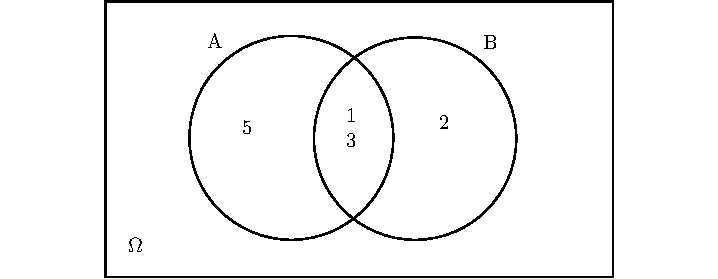
\includegraphics[width=0.9\linewidth]{Livro_files/figure-latex/venndiag-1} 

}

\caption{Exemplo}\label{fig:venndiag}
\end{figure}

\hypertarget{sem2}{%
\chapter{Semana 2}\label{sem2}}

\hypertarget{princuxedpio-aditivo-e-multiplicativo}{%
\section{Princípio aditivo e multiplicativo}\label{princuxedpio-aditivo-e-multiplicativo}}

\begin{definition}[Princípio aditivo]
\protect\hypertarget{def:defAaditivo}{}{\label{def:defAaditivo} \iffalse (Princípio aditivo) \fi{} }Se \(A\) e \(B\) são dois conjuntos disjuntos (\(A \cap B = \emptyset\)) com \(p\) e \(q\) elementos, respectivamente, então \(A \cup B\) possui \(p + q\) elementos.
\end{definition}

\begin{example}
\protect\hypertarget{exm:unnamed-chunk-16}{}{\label{exm:unnamed-chunk-16} }Suponha que tenham entrado em cartaz 3 filmes e 2 peças de teatro, e que Marcelo tenha dinheiro para assistir apenas 1 evento.
Quantos são os programas que Marcelo pode escolher fazer?
\end{example}

\begin{solution}
\iffalse{} {Solução. } \fi{}Defina \[A = \{x \vert x \text{ é filme}\} = \{F_1, F_2, F_3\}\]
e
\[B = \{y \vert y \text{ é teatro}\} = \{T_1, T_2\}.\]
Então,
\[A \cup B = \{x \vert x \text{ é filme ou peça}\}.\]
\(\vert A \vert = 3\) e \(\vert B \vert = 2\), logo \(\vert A \cup B \vert = 5\).
\end{solution}

\begin{definition}[Princípio multiplicativo]
\protect\hypertarget{def:defMultiplicativo}{}{\label{def:defMultiplicativo} \iffalse (Princípio multiplicativo) \fi{} }Se um evento \(A\) pode ocorrer de \(m\) maneiras diferentes, outro evento \(B\) pode ocorrer de \(n\) maneiras diferentes, então o número dew maneiras de ocorrer o evento \(A\) seguido de \(B\) é \(m\times n\).
Em conjuntos, se \(|A|=m\) e \(|B|=n\), então \(|A\times B| = m \times n\).
\end{definition}

\begin{example}
\protect\hypertarget{exm:unnamed-chunk-18}{}{\label{exm:unnamed-chunk-18} }No exemplo anterior, se Marcelo tiver dinheiro para assitir a um filme e a uma peça de teatro, quantos sas os programas que ele pode escolher fazer?
\end{example}

\begin{solution}
\iffalse{} {Solução. } \fi{}\(|A|=3\) e \(|B|=2\).
Também, \(|A\cap B| = \emptyset\).
Então, \(|A \times B| = 6.\)
\end{solution}

\hypertarget{extensuxe3o-do-princuxedpio-aditivo}{%
\subsubsection*{Extensão do princípio aditivo}\label{extensuxe3o-do-princuxedpio-aditivo}}
\addcontentsline{toc}{subsubsection}{Extensão do princípio aditivo}

Se \(A_1, A_2, \ldots, A_n\) são conjuntos, disjuntos 2 a 2, e se \(A_i\) possui \(a_i\) elementos, então a união \(\bigcup_{i=1}^{n}A_i\) possui \(\sum_{i=1}^{n}a_i\) elementos.

\hypertarget{extensuxe3o-do-princuxedpio-multiplicativo}{%
\subsubsection*{Extensão do princípio multiplicativo}\label{extensuxe3o-do-princuxedpio-multiplicativo}}
\addcontentsline{toc}{subsubsection}{Extensão do princípio multiplicativo}

Se um evento \(A_i\) pode ocorrer de \(m_i\) maneiras diferentes, \(i = 1,2,\ldots, n\), então esses \(n\) eventos podem ocorrer, em sucessão, de \(m_1 \times m_2 \times \cdots \times m_n\) maneiras diferentes.

Em linguagem de conjuntos, se \(A_1, A_2, \ldots, A_n\) são conjuntos finitos com \(|A_i|=m_i\), \(i = 1,2,\ldots, n\), então, se \(A_i \cap A_j = \emptyset\), \(i \neq j\),
\[ |A_1 \cup A_2 \cup \cdots \cup A_n| =  \sum_{i=1}^{n}|A_i|,\]
\[ |A_1 \times A_2 \times \cdots \times A_n| =  \prod_{i=1}^{n}|A_i|.\]

\hypertarget{aplicauxe7uxf5s-dos-princuxedpios-aditivo-e-multiplicativo}{%
\subsection{Aplicaçõs dos Princípios Aditivo e Multiplicativo}\label{aplicauxe7uxf5s-dos-princuxedpios-aditivo-e-multiplicativo}}

\begin{example}
\protect\hypertarget{exm:unnamed-chunk-20}{}{\label{exm:unnamed-chunk-20} }Um amigo mostrou-me 5 livros diferentes de matematica, 7 de física e 10 de química e pediu-me para escolher dois livros com a condição de que eles não fossem da mesma matéria. De quantas maneras posso escolhê-los?
\end{example}

\begin{solution}
\iffalse{} {Solução. } \fi{}Posso fazer as seguintes escolhas:

\[ \left.\begin{array}{ll}
\text{a)}& \text{Matemática e física: } 5 \times 7 = 35 \text{ maneiras;} \\ 
\text{b)}& \text{Matemática e química: } 5 \times 10 = 50 \text{ maneiras;} \\ 
\text{c)}& \text{Física e química: } 7 \times 10 = 70 \text{ maneiras.}
\end{array}\right\} \text{(princípio multiplicativo)}
\]

Como minhas escolhas só podem ocorrer dentre uma das possibilidades a), b) ou c), então, pelo princípio aditivo, \(35 + 50 + 70 = 155\) é o número de maneiras de fazer essas escolhas.
\end{solution}

\begin{example}
\protect\hypertarget{exm:unnamed-chunk-22}{}{\label{exm:unnamed-chunk-22} }Quantos são os números que podemos formar com todos os dígitos \(1, 1, 1, 1, 1, 1, 1, 2, 3\)?
\end{example}

\begin{solution}
\iffalse{} {Solução. } \fi{}Se, primeiramente, colocarmos todoos os dígitos \(1\)´s, deixando um espaço entre eles, teremos
\[\_1\_1\_1\_1\_1\_1\_1\_.\]
Há \(8\) espaçoes nos quais podem ser colocador os dígitos \(2\) e \(3\).
Se colocarmos o \(2\) primeiro, uma entre as 8 possibilidades é
\[\_1\_2\_1\_1\_1\_1\_1\_1\_.\]
Agora há \(9\) espaços onde o dígito \(3\) pode ser colocado.
Portanto, \(8 \times 9 = 72\) são os números formados com 9 dígitos, sendo sete \(1\)'s, um 2 e um 3.
\end{solution}

\begin{example}
\protect\hypertarget{exm:unnamed-chunk-24}{}{\label{exm:unnamed-chunk-24} }Há 12 mulheres e 10 homens, 5 deles (3 mulheres e 2 homens) são irmãos e os restantes não possuem parentesco.
Quantos são os casamentos heterosexuais possíveis?
\end{example}

\begin{solution}
\iffalse{} {Solução. } \fi{}

\begin{itemize}
\tightlist
\item
  Considerando as 3 mulheres que possuem irmãos (2), ha \(3\times 8=24\) casamentos possíveis;
\item
  Considerando as 9 mulheres que não possuem irmãos, há \(9\times 10=90\) casamentos possíveis;
\end{itemize}

portanto, pelo princípio aditivo, há \(24+90 = 114\) casamentos heterosexuais possíveis.
\end{solution}

\hypertarget{permutauxe7uxe3o}{%
\section{Permutação}\label{permutauxe7uxe3o}}

\begin{definition}[Permutação]
\protect\hypertarget{def:defPermutacao}{}{\label{def:defPermutacao} \iffalse (Permutação) \fi{} }Uma permutação de \(n\) objetos distintos é qualquer agrupamento ordenado desses objetos, de modo que, se denominarmos \(P_n\) o número das permutações simples dos \(n\) objetos, então
\[P_n = n(n-1)(n-2)\cdots 1 = n!.\]
\end{definition}

\begin{example}
\protect\hypertarget{exm:exPosicoes}{}{\label{exm:exPosicoes} }considerando os digitos \(1, 2, 3, 4\) e \(5\), quantos números de 2 algarismos distintos podem ser formados?
\end{example}

\begin{solution}
\iffalse{} {Solução. } \fi{}Existem duas posiçoes a serem preenchidas \([\text{Pos}_1][\text{Pos}_2]\).
A posição \([\text{Pos}_1]\) pode ser preenchida de 5 maneiras diferentes, restando, portanto, 4 dígitos que podem ocupar a posição \([\text{Pos}_2]\).
Então há \(5\times 4 = 20\) números de 2 algarismos distintos que podem ser formados com os 5 digitos disponíveis.
\end{solution}

\begin{example}
\protect\hypertarget{exm:exConjunto15}{}{\label{exm:exConjunto15} }Dado o conjunto \(A = \{1,2,3,4,5\}\), quantos subconjuntos de 2 elementos \(A\) possui?
\end{example}

\begin{solution}
\iffalse{} {Solução. } \fi{}Vamos listar:
\[
  \left.\begin{matrix}
A_1 = \{1,2\}, & A_2 = \{1,3\},\\ 
A_3 = \{1,4\}, & A_4 = \{1,5\},\\ 
A_5 = \{2,3\}, & A_6 = \{2,4\},\\ 
A_7 = \{2,5\}, & A_9 = \{3,4\},\\ 
A_9 = \{3,5\}, & A_{10} = \{4,5\}. 
\end{matrix}\right.
\]
Ao todo são 10 subconjuntos de 2 elementos formados com os 5 elementos de \(A\).
\end{solution}

\emph{Atenção!} No Exemplo \ref{exm:exPosicoes}, obtivemos 20 números de 2 algarismos diferentes e no Exemplo \ref{exm:exConjunto15} obtivemos 10 subconjuntos de 2 elementos.
Observe que \(12 \neq 21\), mas \(\{1,2\}=\{2,1\}\).
Pelo princípio multiplicativo, obtivemos \(5\times 4=20\), considerando a ordem de colocação dos dígitos.
Na formação de subconjuntos a ordem não importa, devemos dividir o resultado anterior por \(2 = 2\times 1 = 2!\), isto é, pela permutação de 2 que é o número de elementos em cada subconjunto.

\begin{example}
\protect\hypertarget{exm:unnamed-chunk-28}{}{\label{exm:unnamed-chunk-28} }Quantos subconjuntos possui o conjunto \(A = \{a,b,c\}\)?
\end{example}

\begin{solution}
\iffalse{} {Solução. } \fi{}Vamos listar: \(\emptyset, \{a\}, \{b\}, \{c\}, \{a,b\}, \{a,c\}, \{b,c\}, \{a,b,c\}\).
Ao todo há 8 subconjuntos.
Em relação aos elementos, podemos dizer que cada um deles \textbf{aparece} ou \textbf{não aparece} nos subconjuntos.
Então, para o elemento \(a\) temos 2 possibilidades quanto à sua presença no subconjunto (aparecer ou não).
O mesmo para \(b\) e \(c\).
Pelo princípio multiplicativo, temos \(2 \times 2 \times 2 = 8\) subconjuntos de \(A\).
\end{solution}

\begin{example}
\protect\hypertarget{exm:unnamed-chunk-30}{}{\label{exm:unnamed-chunk-30} }Quantos subconjuntos possui um conjunto \(A\) com \(n\) elementos?
\end{example}

\begin{solution}
\iffalse{} {Solução. } \fi{}Pelo exemplo anterior, cada elemento de \(A\) pode ou não estar presente num determinado subconjunto e, pelo fato de \(A\) ter \(n\) elementos, então \(A\) possui \(2\times 2 \times \cdots \times 2 = 2^{n}\) subconjuntos.
\end{solution}

\begin{example}
\protect\hypertarget{exm:unnamed-chunk-32}{}{\label{exm:unnamed-chunk-32} }De quantos modos podemos formar uma roda com 5 crianças?
\end{example}

\begin{solution}
\iffalse{} {Solução. } \fi{}Parece que para formar a roda com as crianças basta escolher uma ordem para elas, o que pode ser feito de \(5!=120\) modos.
Mas veja, na Figura \ref{fig:figRoda}, que as rodas \(ABCDE\) e \(EABCD\) são iguais, pois em uma roda o que importa é a posição relativa das crianças entre si.
A roda \(ABCDE\) pode ser girada para se tornar \(EABCD\).
Como cada roda pode ser girada de 5 formas, a nossa contagem de 120 rodas contou cada uma delas 5 vezes, assim, a resposta é \(120/5=24\).
\end{solution}

--\textgreater{}

\begin{figure}

{\centering 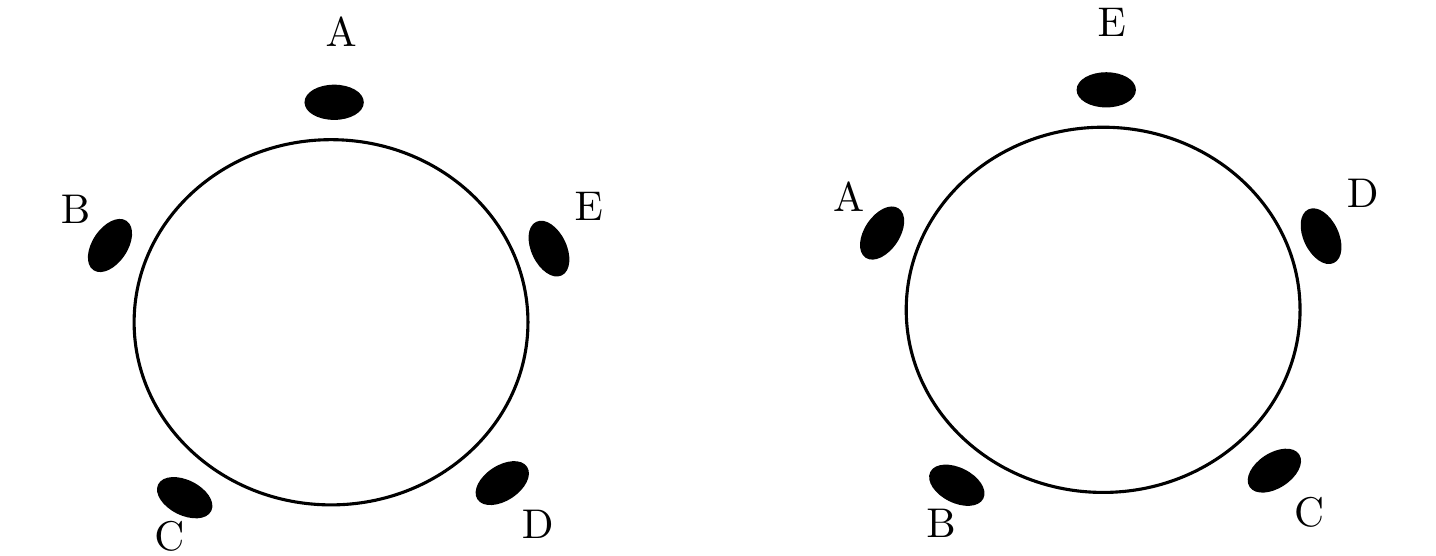
\includegraphics[width=0.9\linewidth]{Livro_files/figure-latex/figRoda-1} 

}

\caption{Roda com cinco crianças.}\label{fig:figRoda}
\end{figure}

\begin{example}
\protect\hypertarget{exm:unnamed-chunk-34}{}{\label{exm:unnamed-chunk-34} }De quantos modos podemos dividir 8 pessoas em dois grupos de 4 pessoas cada?
\end{example}

\begin{solution}
\iffalse{} {Solução. } \fi{}Vamos colocar as 8 pessoas em fila e dividi-las de modo que um grupo seja formado pelas 4 primeiras e o outro pelas 4 últimas.
Como há \(8!\) modos de colocá-las na fila, a resposta parece ser \(8!\).
Considere a divisão \(abcd|efgh\).
Note que ela é idêntica à \(efgh|abcd\).
Na nossa contagem de \(8!\), essas divisões foram contadas como se fossem distintas.
Também, divisões como \(abcd|efgh\) e \(cabd|efgh\), que diferem-se pela ordem dos elementos em cada grupo, foram contadas como se fossem distintas.
Cada divisão foi contada \(2\times 4!\times 4!\) vezes (\(2\) por causa da ordem dos grupos, \(4!\) por causa da ordem dos elementos no primeiro grupo e \(4!\) por causa da ordem dos elementos no segundo grupo).
Assim, o número de divisões é
\[\frac{8!}{2\cdot 4!4!}=35.\]
\end{solution}

\begin{example}
\protect\hypertarget{exm:unnamed-chunk-36}{}{\label{exm:unnamed-chunk-36} }Quantos são os divisores do número 126.000?
\end{example}

\begin{solution}
\iffalse{} {Solução. } \fi{}Ao fatorá-lo, obtemos \(N=126000=2^4\cdot 3^2\cdot 5^2\cdot 7\).
Note que nos divisores de \(N\)

\begin{itemize}
\tightlist
\item
  o expoente do fator \(2\) pode variar de 0 a 4 (\(2^0, 2^1, 2^2, 2^3, 2^4\));
\item
  o expoente do fator \(3\) pode variar de 0 a 2 (\(3^0, 3^1, 3^2\));
\item
  o expoente do fator \(5\) pode variar de 0 a 3 (\(5^0, 5^1, 5^2, 5^3\));
\item
  o expoente do fator \(7\) pode variar de 0 a 1 (\(7^0, 7^1\)).
\end{itemize}

Então, representando os divisores de \(N\) como números da forma

\[D = 2^x\cdot 3^y\cdot 5^z\cdot 7^w,\]

podemos dizer que

\begin{itemize}
\tightlist
\item
  \(x\) toma valores em \(\{0,1,2,3,4\}\), i.e.~\(5\) possibilidades para \(x\);
\item
  \(y\) toma valores em \(\{0,1,2\}\), i.e.~\(3\) possibilidades para \(y\);
\item
  \(z\) toma valores em \(\{0,1,2,3\}\), i.e.~\(4\) possibilidades para \(z\);
\item
  \(w\) toma valores em \(\{0,1\}\), i.e.~\(2\) possibilidades para \(w\).
\end{itemize}

Assim, pelo princípio multiplicativo, \(5\cdot 3\cdot 4\cdot 2 = 120\) divisores de \(N\).
\end{solution}

\hypertarget{arranjo-simples-r-permutauxe7uxe3o}{%
\section{\texorpdfstring{Arranjo simples (\(r\)-permutação)}{Arranjo simples (r-permutação)}}\label{arranjo-simples-r-permutauxe7uxe3o}}

\begin{definition}[Arranjo simples]
\protect\hypertarget{def:defArranjo}{}{\label{def:defArranjo} \iffalse (Arranjo simples) \fi{} }Um arranjo simples de \(n\) elementos tomandos \(r\) a \(r\), em que \(n \geq 1\) e \(r \leq n\), \(r \in \mathbf{R}\) são todos os grupos de \(r\) elementos distrintos que diferem entre si pela ordem e pela natureza dos \(r\) elementos que compõem cada grupo.
Notação: \(A^{r}_{n}\).
\end{definition}

Vamos encontrar uma expressão matemática que caracterize \(A^{r}_{n}\).
Temos \(n\) elementos dos quais queremos tomar \(r\).
Isto equivale a preencher \(r\) lugares com \(n\) objetos.

\[
\underbrace{\_\_}_{L_1}\underbrace{\_\_}_{L_2}\underbrace{\_\_}_{L_3}\cdots\underbrace{\_\_}_{L_r}
\]

No primeiro lugar há \(n\) objetos diferentes que podem ser escolhidos.
No segundo lugar há \(n-1\) objetos diferentes (lembre-se que um já foi escolhido).
No terceiro lugar há \(n-2\) objetos diferentes, e assim sucessivamente, de forma que \(L_r\) terá \(n-(r-1)\) maneiras diferentes de ser preenchido.
Pelo Princípio Multiplicativo, podemos dizer que as \(r\) posições podem ser preenchidas sucessivamente de \(n(n-1)(n-2)\cdots(n-(r-1))\) maneiras distintas.
Portanto
\[
A^{r}_{n} = n(n-1)(n-2)\cdots(n-(r-1)).
\]

Multiplicando e dividindo por 1, temos que

\[
A^{r}_{n} = n(n-1)(n-2)\cdots(n-(r-1))\frac{(n-r)(n-r-1)\cdots2\cdot 1}{(n-r)(n-r-1)\cdots2\cdot 1} = \frac{n!}{(n-r)!}.
\]

\begin{example}
\protect\hypertarget{exm:unnamed-chunk-38}{}{\label{exm:unnamed-chunk-38} }Quantos inteiros entre 1000 e 9999 tem dígitos distintos e
(a) são números pares?
(b) constituem-se inteiramente de dígitos ímpares?
\end{example}

\begin{solution}
\iffalse{} {Solução. } \fi{}Os números que buscamos tem 4 dígitos, ou 4 posições a serem preenchidas

\[
  \underbrace{\_\_}_{p_1}\underbrace{\_\_}_{p_2}\underbrace{\_\_}_{p_3}\underbrace{\_\_}_{p_4}.
\]

Para resolver o item (a), note que números pares tem na última posição 0, 2, 4, 6 ou 8.

\begin{itemize}
\item
  números terminados em 0: \(\underbrace{\_\_}_{p_1}\underbrace{\_\_}_{p_2}\underbrace{\_\_}_{p_3}\underbrace{0}_{p_4}\).
  Com excessão do zero, dígitos disponíveis: \(1,2,\ldots,9\).
  Preenchemos as três primeiras posiçõeos de \(A^{3}_{9}=\frac{9!}{6!}=504\) maneiras.
\item
  números terminados em 2, 4, 6 ou 8:
  Preenchimento da última posição: 4 maneiras.
  Preenchimento da primeira posição: 8 maneiras (exclui-se 0 e o dígito em \(p_4\)).
  Preenchemos as posições \(p_2\) e \(p_3\) de \(A^{2}_{8}=\frac{8!}{6!}=56\) maneiras.
  Pelo Princípio Multiplicativo, há \(4\cdot 8\cdot A^{2}_{8} = 1792\) números pares com dígitos distintos que não terminam em zero.
\end{itemize}

Finalmente, pelo Princípio Aditivo, há \(A^{3}_{9} + 4\cdot 8 \cdot A^{3}_{9} = 2296\) números pares entre 1000 e 9999 com dígitos distintos.

No item (b), se os números são constituidos de dígitos ímpares, então são formados pelos dígitos 1, 3, 5, 7 e 9.
Portanto há \(A^4_5=5!=120\) números entre 1000 e 9999 formados de dígitos ímpares.
\end{solution}

\hypertarget{combinauxe7uxf5es}{%
\section{Combinações}\label{combinauxe7uxf5es}}

\begin{definition}[Combinação simples]
\protect\hypertarget{def:defComb}{}{\label{def:defComb} \iffalse (Combinação simples) \fi{} }Combinações simples de \(n\) elementos tomados \(r\) a \(r\) (\(r\)-combinação), em que \(n \geq 1\), \(r \in \mathbb{N}\) tal que \(r \leq n\), são todas as escolhas não ordenadas de \(r\) desses elementos.
Notação \(C^r_n = {n\choose r}\).
\end{definition}

\begin{example}
\protect\hypertarget{exm:unnamed-chunk-40}{}{\label{exm:unnamed-chunk-40} }Seja \(\mathcal{S} = \{1,2,3,4\}\).
O subconjunto \(\{1,3,4\}\) é uma \(3\)-combinação do conjunto \(\mathcal{S}\).
Note que \(\{4,1,3\}\) é a mesma \(3\)-combinação, pois a ordem em que os elementos são listados não importa.
\end{example}

\begin{example}
\protect\hypertarget{exm:unnamed-chunk-41}{}{\label{exm:unnamed-chunk-41} }Considere o conjunto \(\mathcal{X}_1 = \{1,2,3\}\), um conjunto de cardinalidade \(3\).
Quais são todos os subconjuntos de \(\mathcal{X}_1\)?
\end{example}
\begin{solution}
\iffalse{} {Solução. } \fi{}O conjunto vazio é o único subconjunto de \(\mathcal{X_1}\) com tamanho zero.
Existem \(3\) subconjuntos de tamanho \(1\),
\[ \{1\}, \qquad \{2\}, \qquad \{3\}. \]
Também existem \(3\) subconjuntos de tamanho \(2\),
\[ \{1,2\}, \qquad \{1,3\}, \qquad \{2,3\}. \]
E existe \(1\) subconjunto de tamanho 3, o próprio \(\mathcal{X}_1\).
\end{solution}

\begin{example}
\protect\hypertarget{exm:exComb4}{}{\label{exm:exComb4} }Considere agora \(\mathcal{X}_2 = \{1,2,3,4\}\).
Quais são todos os subconjuntos de \(\mathcal{X}_2\)?
\end{example}

\begin{solution}
\iffalse{} {Solução. } \fi{}Novamente, o conjunto vazio é o único subconjunto de \(\mathcal{X}_2\) com tamanho zero e \(\mathcal{X}_2\) é o único subconjunto de tamanho \(4\).
Existem \(4\) subconjuntos de tamanho \(1\),
\[ \{1\}, \qquad \{2\}, \qquad \{3\}, \qquad \{4\}. \]
Também existem \(6\) subconjuntos de tamanho \(2\),
\[ \{1,2\}, \qquad \{1,3\}, \qquad \{1,4\}, \]
\[ \{2,3\}, \qquad \{2,4\}, \qquad \{3,4\}. \]
E existem \(4\) subconjuntos de tamanho 3,
\[ \{1,2,3\}, \qquad \{1,2,4\}, \qquad \{1,3,4\}, \qquad \{2,3,4\}.\]
\end{solution}

Note que, no Exemplo \ref{exm:exComb4}, os conjuntos de tamanho \(3\) são uma bijeção entre os conjuntos de tamanho \(1\), já que todo conjunto de tamanho \(3\) é o complemento de conjunto de tamanho \(1\).
Em geral, é verdade que o número de subconjuntos com \(k\) elementos é igual ao número de subconjuntos com \(n-k\) elementos.

\begin{proposition}
\protect\hypertarget{prp:unnamed-chunk-44}{}{\label{prp:unnamed-chunk-44} }Para todo \(n \in \mathbb{N}\) e todo \(k \in \mathbb{Z}\), se \({n \choose k}\) denota o número de subconjuntos de cardinalidade \(k\) de um conjunto de cardinalidade \(n\), então
\begin{align}
{0 \choose 0} &= 1, \\
{n \choose k} &= 0, \qquad \text{se } k \notin \{0, 1, \cdots, n\},\\
{n \choose k} &= {n-1 \choose k} + {n-1 \choose k-1}.
\end{align}
\end{proposition}

\begin{proof}
\iffalse{} {Prova. } \fi{}Claramente, quando \(k \notin \{0, 1, \cdots, n\}\), temos que \({n \choose k} = 0\).
Temos também que \({0 \choose 0} = 1\), pois o conjunto vazio é o único subconjunto de tamanho zero.
Se \(n\geq 1\), temos que considerar os casos em que \(k=0\) e \(k=n\) separadamente.

\begin{itemize}
\item
  Se \(k=0\), então o único subconjunto de \(\{0, 1, \ldots, n\}\) com zero elementos é o conjunto vazio, assim
  \[ {n \choose 0} = 1 = {n-1 \choose 0} + {n-1 \choose -1} = 1+0.\]
\item
  Se \(k=n\), então o único subconjunto de \(\{0, 1, \ldots, n\}\) com \(n\) elementos é o próprio \(\{0, 1, \ldots, n\}\), assim,
  \[ {n \choose n} = 1 = {n-1 \choose n} + {n-1 \choose n-1} = 0+1.\]
\item
  Se \(1 \leq k \leq n-1\), então existem dois tipos de subconjuntos de \(\{0, 1, \cdots, n\}\) com \(k\) elementos: aqueles que contém n e aqueles que não contém \(n\).
  O número de subconjuntos de \(k\) elementos de \(\{0, 1, \ldots, n\}\) contendo \(n\) é igual ao número de subconjuntos de \(\{0, 1, \ldots, n\}\) contendo \(k-1\) elementos, que é denotado por \({n-1 \choose k-1}\).
  O número de subconjuntos de \(k\) elementos de \(\{0, 1, \ldots, n\}\) que não contém \(n\) é igual ao número de subconjuntos de \(\{0, 1, \ldots, n\}\) contendo \(k\) elementos, que é denotado por \({n-1 \choose k}\).
  Então, o número de subconjuntos de \(\{0, 1, \ldots, n\}\) com \(k\) elementos é
  \[ {n \choose k} = {n-1 \choose k} + {n-1 \choose k-1}.\]
\end{itemize}

A equação acima é conhecida também com \href{https://pt.wikipedia.org/wiki/Rela\%C3\%A7\%C3\%A3o_de_Stifel}{relação de Stifel}, ou regra de Pascal.
\end{proof}

FALAR MAIS SOBRE O TRIANGULO DE PASCAL

\begin{figure}

{\centering 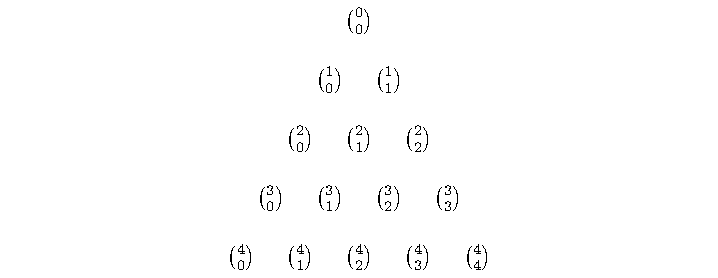
\includegraphics[width=0.9\linewidth]{Livro_files/figure-latex/unnamed-chunk-46-1} 

}

\caption{Triângulo de Pascal.}\label{fig:unnamed-chunk-46}
\end{figure}

\begin{example}
\protect\hypertarget{exm:unnamed-chunk-47}{}{\label{exm:unnamed-chunk-47} }\[{4 \choose 1} = {3 \choose 0} + {3 \choose 1},\]
\[{4 \choose 2} = {3 \choose 2} + {3 \choose 1}.\]
\end{example}

\begin{proposition}
\protect\hypertarget{prp:unnamed-chunk-48}{}{\label{prp:unnamed-chunk-48} }Para todo \(n \in \mathbb{N}\) e todo \(k \in \mathbb{Z}\), \(0 \leq k \leq n\), temos
\[{n \choose k} = \frac{n!}{k!(n-k)!}.\]
\end{proposition}

\begin{proof}
\iffalse{} {Prova. } \fi{}Vamos usar indução sobre n para fazer a prova.

\begin{enumerate}
\def\labelenumi{\arabic{enumi}.}
\item
  Para \(n=0\). Como \(0 \leq k \leq n\), temos que \(k=0\), logo \({0 \choose 0} =1\),
  \[\frac{0!}{0!(0)!}=1.\]
\item
  Hipótese de indução: supor que se cumpre para n-1.
\item
  Verificar que vale para \(n\).
\end{enumerate}

Pela fórmula de Pascal
\begin{align}
{n \choose k} &= {n-1 \choose k} + {n-1 \choose k-1} \\
&= \frac{(n-1)!}{k!(n-1-k)!} + \frac{(n-1)!}{(k-1)!(n-1-(k-1))!} \\
&= \frac{(n-1)!}{k!(n-1-k)!} + \frac{(n-1)!}{(k-1)!(n-k)!} \\
&= \frac{(n-k)}{(n-k)}\frac{(n-1)!}{k!(n-1-k)!} + \frac{k}{k}\frac{(n-1)!}{(k-1)!(n-k)!} \\
&= \bigg(\frac{n-k}{k!(n-k)(n-k-1)!} + \frac{k}{k(k-1)!(n-k)!} \bigg)(n-1)! \\
&= \bigg(\frac{n-k}{k!(n-k)!} + \frac{k}{k!(n-k)!} \bigg)(n-1)! \\
&= \frac{n}{k!(n-k)!}(n-1)! \\
&= \frac{n!}{k!(n-k)!}.
\end{align}
\end{proof}

\begin{example}
\protect\hypertarget{exm:unnamed-chunk-50}{}{\label{exm:unnamed-chunk-50} }Quantos são os anagramas formados por \(2\) vogais e \(3\) consoantes escolhidas dentre \(18\) consoantes e \(5\) vogais?
\end{example}

\begin{solution}
\iffalse{} {Solução. } \fi{}A escolha das duas vogais pode se dar de \(C^2_5\) maneiras diferentes.
A escolha das consoantes pode se dar de \(C^3_{18}\) maneiras diferentes.
Portanto, pelo Princípio Multiplicativo, o número de anagramas possíveis formados por \(2\) vogais e \(3\) consoantes é
\[C^2_5 \cdot C^3_{18} = \frac{5!}{2!3!}\frac{18!}{3!15!}=8160.\]
\end{solution}

\begin{remark}
\iffalse{} {Observação. } \fi{}Por simetria, \(C^{k}_{n} = C^{n-k}_n\).
O número \(C^{n-k}_n\) é chamado de combinação complementar.
Isto é, se consideramos um conjunto com \(n\) elementos, o número de maneiras de escolher \(k\) objetos é identico ao número de maneiras de escolher \(n-k\) objetos dentre os \(n\), pois do total \(n\) tiramos \(k\) e sobram \(n-k\) e, consequentemente, se de \(n\) objetos tiramos \(n-k\), sobram-se \(k\) objetos.
\end{remark}

\begin{example}
\protect\hypertarget{exm:unnamed-chunk-53}{}{\label{exm:unnamed-chunk-53} }De quantas maneiras podemos arrumar em fila \(5\) sinais negativos \((-)\) e \(7\) sinais positivos \((+)\)?
\end{example}

\begin{solution}
\iffalse{} {Solução. } \fi{}Este problema é equivalente à ter \(12\) lugares para se preencher com sinais \(-\) e \(+\).
Neste caso, tanto faz se escolhermos \(5\) lugares dentre os \(12\) para colocar os \(-\) e nos que sobrarem colocarmos os \(7\) \(+\), ou o contrário, visto que \(C^{5}_{12} = C^{7}_{12} = \frac{12!}{7!5!}=792.\)
\end{solution}

\begin{example}
\protect\hypertarget{exm:unnamed-chunk-55}{}{\label{exm:unnamed-chunk-55} }Quantas diagonais possui um polígono regular de \(n\) lados?
\end{example}

\begin{solution}
\iffalse{} {Solução. } \fi{}Sejam \(P_1, P_2, \cdots, P_n\) os vértices.
Ao observar a Figura \ref{fig:figPoligono}, vemos que não pode-se ligar \(P_1\) a \(P_2\) e nem \(P_1\) a \(P_8 (=P_n)\), pois teríamos lados e não diagonais.
Entretanto, \(P_1\) pode ser ligado a qualquer um dos \(5 = n-3\) vértices restantes.
O número de maneiras de traçarmos estas diagonais é escolher 1 dentre os \(n-3\) vértices restantes, isto é \(C^{1}_{n-3}\).
Como há \(n\) vértices e para cada um deles há \(C^{1}_{n-3}\) diagonais possíveis, então \(n \cdot C^{1}_{n-3}\) deveria ser o número de diagonais do polígono.
Mas estaríamos contando a diagonal entre os vértices \(P_1\) e \(P_3\), por exemplo, duas vezes.
Devemos então dividir este resultado por \(2\).
Portanto, um polígono regular de \(n\) lados possui
\[ \frac{n \cdot C^{1}_{n-3}}{2} = \frac{n}{2}\frac{(n-3)!}{1!(n-4)!} = \frac{n(n-3)}{2} \]
diagonais.
\end{solution}

\begin{figure}

{\centering 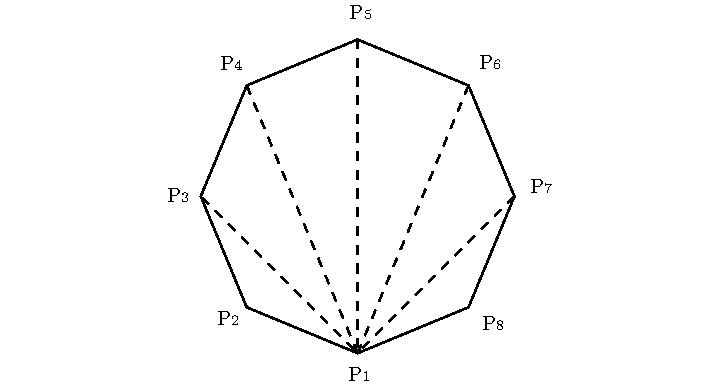
\includegraphics[width=0.9\linewidth]{Livro_files/figure-latex/figPoligono-1} 

}

\caption{Polígono regular de 8 lados.}\label{fig:figPoligono}
\end{figure}

\begin{example}
\protect\hypertarget{exm:unnamed-chunk-57}{}{\label{exm:unnamed-chunk-57} }De quantas maneiras pode-se escolher \(3\) números distintos do conjunto \(\mathcal{A}=\{1, 2, 3, \ldots, 50\}\) de modo que sua soma seja um múltiplo de \(3\)?
\end{example}

\begin{solution}
\iffalse{} {Solução. } \fi{}Sejam os conjuntos

\begin{align}
\mathcal{A}_1 &= \{x \in \mathcal{A} | x=3k, k=1,2,\ldots \} = \{3, 6, 9, \ldots, 48\},\\
\mathcal{A}_2 &= \{x \in \mathcal{A} | x=3k+1, k=1,2,\ldots \} = \{1, 4, 7, 10, \ldots, 49\},\\
\mathcal{A}_3 &= \{x \in \mathcal{A} | x=3k+2, k=1,2,\ldots \} = \{2, 5, 8, 11, \ldots, 50\}.\\
\end{align}

Vamos denominar \(n(\mathcal{A}_i)\) a cardinalidade de \(\mathcal{A}_i\).
Então,
\[n(\mathcal{A}_1) = 16, \qquad n(\mathcal{A}_2)=17, \qquad n(\mathcal{A}_3)=17.\]

Se somarmos \(3\) números quaisquer de \(\mathcal{A}_1\), teremos como soma um múltiplo de \(3\), pois se \(x,y,z \in \mathcal{A}_1\), então \(x+y+z = 3(k + k^{\prime} + k^{\prime\prime})\), em que \(k, k^\prime, k^{\prime\prime} \in \mathbb{N}\).
Essa soma pode ser feita de \(C^{3}_{16} = \frac{16!}{3!13!}=560\) maneiras.

Se somarmos 3 números quaisquer de \(\mathcal{A}_2\), teremos como soma um múltiplo de \(3\), pois se \(x,y,z \in \mathcal{A}_2\), então \(x+y+z =(3k+1)+(3k^{\prime}+1)+(3k^{\prime\prime}+1)=3(k + k^{\prime} + k^{\prime\prime})+3\), em que \(k, k^\prime, k^{\prime\prime} \in \mathbb{N}\).
Essa soma pode ser feita de \(C^{3}_{17} = \frac{17!}{3!14!}=680\) maneiras.

Se somarmos 3 números quaisquer de \(\mathcal{A}_3\), teremos como soma um múltiplo de \(3\), pois se \(x,y,z \in \mathcal{A}_3\), então \(x+y+z =(3k+2)+(3k^{\prime}+2)+(3k^{\prime\prime}+2)=3(k + k^{\prime} + k^{\prime\prime})+6\), em que \(k, k^\prime, k^{\prime\prime} \in \mathbb{N}\).
Essa soma pode ser feita de \(C^{3}_{17} = \frac{17!}{3!14!}=680\) maneiras.

Se somarmos \(1\) elemento de \(\mathcal{A}_1\) com \(1\) elemento de \(\mathcal{A}_2\) e com \(1\) elemento de \(\mathcal{A}_3\), obteremos como soma um múltiplo de \(3\), pois se \(x \in \mathcal{A}_1\), \(y \in \mathcal{A}_2\) e \(z \in \mathcal{A}_3\), então \(x+y+z =\) \(3k+(3k^{\prime}+1)+(3k^{\prime\prime}+2)=\) \(3(k + k^{\prime} + k^{\prime\prime})+3\), em que \(k, k^\prime, k^{\prime\prime} \in \mathbb{N}\).
Essa soma pode ser feita de \(C^{1}_{16}C^{1}_{17}C^{1}_{17} = 16 \cdot 17 \cdot 17 = 4624\) maneiras.

Portanto, podemos escolher \(3\) números distintos de \(\mathcal{A}\), de modo a obter um múltiplo de \(3\), de \(C^{3}_{16}+C^{3}_{17}+C^{3}_{17}+C^{1}_{16}C^{1}_{17}C^{1}_{17} = 6544\) maneiras.
\end{solution}

\begin{example}
\protect\hypertarget{exm:unnamed-chunk-59}{}{\label{exm:unnamed-chunk-59} }Dado \(A = \{1,2,3,4,5\}\), de quantos modos é possível formar subconjuntos de \(2\) elementos nos quais não haja números consecutivos?
\end{example}

\begin{example}
\protect\hypertarget{exm:exNumConsec}{}{\label{exm:exNumConsec} }Vamos enumerar estes conjuntos: \(\{1,3\}\), \(\{1,4\}\), \(\{1,5\}\), \(\{2,4\}\), \(\{2,5\}\), \(\{3,5\}\).
Há, portanto, \(6\) subconjuntos nas condições impostas pelo enunciado do problema.
\end{example}

Neste caso explorado pelo Exemplo \ref{exm:exNumConsec} foi fácil enumerear.
Entretanto, para um conjunto com \(10\) elementos, a solução não seria tão fácil de ser determinada.
Vamos encontrar uma maneira de contar o número de subconjuntos sem que haja a necessidade de enumerá-los.
Vamos marcar com o sinal ``\(+\)'' os elementos que farão parte do subconjunto e com o sinal ``\(-\)'' os elementos que não farão parte do subconjunto.
Dessa forma, \(\{1,3\}\) pode ser representado por \(+-+--\), \(\{2,5\}\) pode ser representado por \(-+--+\), e \(\{1,2\}\) pode ser representado por \(++---\), que não é um conjunto válido, de acordo com as condições do enunciado.
Veja que para formar o subconjunto desejado, devemos colocar 3 sinais ``\(-\)'' e 2 sinais ``\(+\)'' em fila, sem que haja dois sinais ``\(+\)'' consecutivos.
Isto pode ser feito se colocarmos os \(3\) sinais ``\(-\)'' e deixarmos espaços entre eles, onde eventualmente colocaremos os sinais ``\(+\)''.
\[\_\_ - \_\_ - \_\_ - \_\_ .\]
Há \(4\) posições vazias, e, para colocarmos os dois sinais ``\(+\)'', basta escolhermos \(2\) dentre estas \(4\) posições.
Consequentemente, há \(C^2_4=6\) maneiras disso ser feito e, portanto, há \(6\) subconjuntos de \(2\) elementos não consecutivos de \(A\).

\hypertarget{aplicauxe7uxf5es}{%
\section{Aplicações}\label{aplicauxe7uxf5es}}

\hypertarget{equauxe7uxf5es-lineares-com-coeficientes-unituxe1rios}{%
\subsection{Equações lineares com coeficientes unitários}\label{equauxe7uxf5es-lineares-com-coeficientes-unituxe1rios}}

O objetivo aqui é contar o número de soluções inteiras de uma equação da forma

\begin{equation}
x_1 + x_2 + x_3 + \cdots + x_n = m,
\label{eq:inteiros}
\end{equation}

em que \(x_i\), para \(i=1,2,\ldots, n\), e \(m\) são inteiros.

\begin{theorem}
\protect\hypertarget{thm:eqIntPos}{}{\label{thm:eqIntPos} }O número de soluções em inteiros positivos da Equação \eqref{eq:inteiros}, para \(m>0\) é dado por \(C^{n-1}_{m-1}\).
\end{theorem}

\begin{proof}
\iffalse{} {Prova. } \fi{}Como estamos interessados em expressar o inteiro positivo \(m\) como soma de \(r\) inteiros positivos, basta colocarmoms \(n-1\) barras divisoras entre os \(m\) \(1\)´s:

\[1 + 1 \vert + 1 + \cdots +1 \vert  +1 \cdots  + 1 \vert + 1 + \cdots + 1 =m.\]

O valor de \(x_1\) será o número de \(1\)´s que antecedem a primeira barra, o valor de \(x_2\) será o número de \(1\)´s entre a primeira e a segunda barra, e assim por diante, até obtermos o valor de \(x_n\) como sendo o número de \(1\)´s à direita da barra de número \(n-1\).
Como a cada possível distribuição das barras corresponde uma única solução para a equação acima, basta contarmos de quantas formas isso pode ser feito.
Devemos selecionar \(n-1\) dos \(m-1\) possíveis locais (os sinais de ``\(+\)'' que separam os \(1\)´s) para a colocação das barras divisórias, o que pode ser feito de \(C^{n-1}_{m-1}\) maneiras diferentes.
\end{proof}

\begin{theorem}
\protect\hypertarget{thm:solNaoNegInt}{}{\label{thm:solNaoNegInt} }O número de soluções não negativas inteiras da Equação \eqref{eq:inteiros}, para \(m>0\) e \(x_i\geq 0\) é dado por \(C^{n-1}_{m+n-1} = C^{m}_{m+n-1}\).
\end{theorem}

\begin{proof}
\iffalse{} {Prova. } \fi{}Somando \(1\) a cada \(x_i\), temos
\[(x_1+1) + (x_2+1) + (x_3+1) + \cdots + (x_n+1) = m+n.\]
Seja \(y_i = x_i+1\), para \(i=1,2,\ldots,n\), então
\begin{equation}
y_1 + y_2 + y_3 + \cdots + y_n = m+n,
\label{eq:inteirosY}
\end{equation}
para \(y_i \geq 1\), inteiro.
Este problema é equivalente a determinar o número de soluções inteiras positivas da Equação \eqref{eq:inteirosY}, que, pelo Teorema \ref{thm:eqIntPos}, é
\[C^{n-1}_{m+n-1} = C^{m}_{m+n-1}.\]
\end{proof}

\begin{example}
\protect\hypertarget{exm:unnamed-chunk-62}{}{\label{exm:unnamed-chunk-62} }Encontrar (a) o número de soluções em inteiros não-negativos e (b) soluções em inteiros positivos da equação \(x_1 + x_2 + x_3 + x_4 + x_5 = 12\).
\end{example}

\begin{solution}
\iffalse{} {Solução. } \fi{}(a) \(C^{5-1}_{12+5-1} = C^{4}_{16} = 1820,\)
(b) \(C^{4}_{11} = 330.\)
\end{solution}

\begin{example}
\protect\hypertarget{exm:unnamed-chunk-64}{}{\label{exm:unnamed-chunk-64} }Encontrar o número de soluções em inteiros positivos maiores do que \(3\) na equação \(x_1 + x_2 + x_3 = 17\), isto é, determinar o número de soluções inteiras de \(x_1 + x_2 + x_3 = 17\), em que \(x_i>3\), \(i=1,2,3\).
\end{example}

\begin{solution}
\iffalse{} {Solução. } \fi{}Algumas soluções procuradas são \((4,5,8)\), \((5,7,5)\) e \((9,4,4)\).
Subtraindo \(3\) unidades de cada componente destas ternas ordenadas, obtemos \((1,2,5)\), \((2,4,2)\) e \((6,1,1)\), respectivamente, que são soluções em inteiros positivos da equação
\begin{equation}
y_1 + y_2 + y_3 = 8, \qquad y_i\geq 1,
\label{eq:inteirosY2}
\end{equation}

em que \(y_i=x_i-3\), \(i=1,2,3\).
Como o número de soluções da Equação \eqref{eq:inteirosY2} é \(C^2_7=21\), este é o número procurado, uma vez que esta mudança de variável descrita acima estabelece uma relação biunívoca entre os conjuntos de soluções das duas equações.
\end{solution}

\hypertarget{combinauxe7uxf5es-com-repetiuxe7uxf5es}{%
\section{Combinações com repetições}\label{combinauxe7uxf5es-com-repetiuxe7uxf5es}}

\begin{example}
\protect\hypertarget{exm:parqueDiversoes}{}{\label{exm:parqueDiversoes} }Num parque de diversões existem quatro tipos de brinquedos, \(a\), \(b\), \(c\) e \(d\).
Uma pessoa quer comprar dois bilhetes.
De quantas maneiras ela pode comprar?
\end{example}

\begin{solution}
\iffalse{} {Solução. } \fi{}É claro que ela pode comprar dois bilhetes do mesmo tipo.
A lista de possibilidades é

\begin{align}
aa, &\quad ab, \quad ac, \quad ad, \quad bb, \\
bc, &\quad bd, \quad cc, \quad cd, \quad dd. 
\label{eq:combRep}
\end{align}
\$\$\$\$

Veja que este número de possibilidades é maior que \(C^2_4=6\).
\end{solution}

As combinações listadas na Expressão \eqref{eq:combRep} são chamadas combinações com repetição.

Retomando o contexto apresentado no Exemplo \ref{exm:parqueDiversoes}, se uma pessoa tem dinheiro para comprar \(5\) bilhetes, algumas possibilidades seriam

\[aaaaa, \quad abbbc, \quad bbccd.\]
Estamos interessados em contar o total de elementos do tipo acima.
Para saber os bilhetes comprados, basta que a pessoa nos diga quantos bilhetes de cada tipo ela comprou.
Sejam \(x_1, x_2, x_3, x_4\) o número de bilhetes comprados para os brinquedos \(a,b,c,d\), respectivamente.
O que estamos procurando é o número de soluções inteiras não-negativas para a equação
\[x_1+x_2+x_3+x_4=5,\]
que, como sabemos, através do Teorema \ref{thm:solNaoNegInt}, é \(C^3_8=56\), e vamos denotar por \(CR^5_4\).

Podemos generalizar o resultado anterior.
Assim, \(CR^p_n\) é o número total de maneiras de selecionarmos \(p\) objetos dentre \(n\) objetos distintos, em que cada objeto pode ser escolhido até \(p\) vezes, que, como vimos, é igual ao número de soluções não negativas da equação
\[x_1+x_2+\cdots x_p=n,\]
que é \[C^{n-1}_{n+p-1}=C^{p}_{n+p-1}.\]
Logo temos que
\[CR^{p}_{n}=CR^{p}_{n+p-1}.\]

\hypertarget{sem3}{%
\chapter{Semana 3}\label{sem3}}

\hypertarget{princuxedpio-da-inclusuxe3o-e-exclusuxe3o}{%
\section{Princípio da inclusão e exclusão}\label{princuxedpio-da-inclusuxe3o-e-exclusuxe3o}}

Queremos obter uma fórmula que forneça o número total de elementos na união de um número finito de conjuntos.
Considere o diagrama mostrado na Figura \ref{fig:figVennAB}, com os conjuntos \(A\) e \(B\).
O número total de elementos da união \(A \cup B\) é
\[|A\cup B| = |A| + |B| - |A\cap B|.\]

\begin{figure}

{\centering 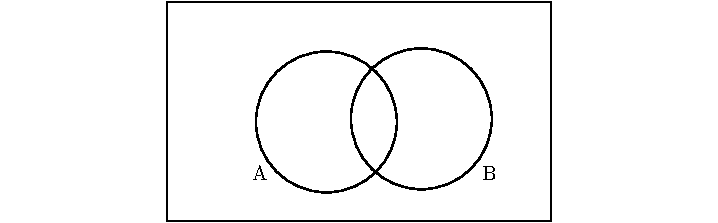
\includegraphics[width=0.9\linewidth]{Livro_files/figure-latex/figVennAB-1} 

}

\caption{Polígono regular de 8 lados.}\label{fig:figVennAB}
\end{figure}

\begin{theorem}
\protect\hypertarget{thm:teoPrincInclExcl}{}{\label{thm:teoPrincInclExcl} }O número de elementos na união de \(n\) conjuntos finitos \(A_1, A_2, \ldots, A_n\) é dado por
\begin{align}
|A_1 \cup A_2 \cap \cdots \cap A_n| = &\sum_{i=1}^{n} |A_i| - \sum_{1\leq i\leq j} |A_i \cap A_j|\\
  &+ \sum_{1\leq i\leq j\leq k} |A_i \cap A_j \cap A_k| + \cdots + (-1)
\label{eq:inclusaoExclusao}
\end{align}
\end{theorem}

\begin{proof}
\iffalse{} {Prova. } \fi{}Devemos mostrar que um elemento que pertença a \(p\) dos conjuntos \(A_i\), para \(p=1,2,\ldots, n\), é contado pela Expressão \eqref{eq:inclusaoExclusao} exatamente uma vez.
Pertencendo a \(p\) dos conjuntos \(A_i\)`s, ele será contato \(p\) vezes em
\[\sum_{i=1}^{n} |A_i|,\]
em
\[\sum_{1\leq i\leq j} |A_i \cap A_j|\]
será contado \(C^2_p\) vezes (há \(C^2_n\) interseções dois a dois e o elemento está em \(C^2_p\) delas),
em
\[\sum_{1\leq i\leq j\leq k} |A_i \cap A_j \cap A_k|\]
será contado \(C^3_p\) vezes, e assim sucessivamente até o termo \(|A_1 \cap A_2 \cap \cdots A_n|\), em que o elemento será contado uma vez.
A interseção de mais do que \(p\) conjuntos não fornecerá nenhuma contribuição, pois o elemento em questão pertence a exatamente \(p\) dos conjuntos \(A_1, A_2, \ldots, A_n\).

Somando todas essas contribuições, teremos

\begin{equation}
C^{1}_{p}-C^{2}_{p}+C^{3}_{p}-C^{4}_{p}+\cdots +(-1)^{p-1}C^{p}_{p}
\label{eq:inclusaoExclusaoFinal}
\end{equation}

Os termos que aparecem na soma da Expressão \eqref{eq:inclusaoExclusaoFinal} são os elementos da \(p\)-ésima linha do triângulo de Pascal.
Sabemos que termos equidistantes dos extremos em uma linha do triângulo de Pascal são iguais (C\^{}\{k\}\emph{\{p\}=C\^{}\{p-k\}}\{p\}), assim

\[C^{0}_{p}-C^{1}_{p}+C^{2}_{p}-C^{3}_{p}+C^{4}_{p}+\cdots +(-1)^{p}C^{p}_{p} = 0.\]
Isso implica que a soma na Expressão \eqref{eq:inclusaoExclusaoFinal} é igual a 1, pois \(C^{0}_{p}=1\).
\end{proof}

A seguir, veremos alguns exemplos de aplicação do Princípio da Inclusão e Exclusão.

\begin{example}
\protect\hypertarget{exm:unnamed-chunk-68}{}{\label{exm:unnamed-chunk-68} }Dentre os números de 1 até 3600 inclusive, quantos são divisíveis por 3 ou por 7?
\end{example}

\begin{solution}
\iffalse{} {Solução. } \fi{}Sabemos que \(\big\lfloor{\frac{3600}{3}}\big\rfloor=1200\) são divisíveis por \(3\) e que \(\big\lfloor{\frac{3600}{7}}\big\rfloor=514\) são divisíveis por 7.
Ao somar estes números estaremos contando duas vezes todos os números que são divisíveis por \(3\) e por \(7\), ou seja, os divisíveis por \(21\), que são \(\big\lfloor{\frac{3600}{21}}\big\rfloor=171\).
Logo, dentre os números de 1 até 3600 inclusive,
\[1200 + 514 - 171 = 1543\]
são divisíveis por 3 ou por 7.
\end{solution}

\begin{example}
\protect\hypertarget{exm:div3Numeros}{}{\label{exm:div3Numeros} }Quantos são os inteiros entre 1 até 42000 inclusive que não são divisíveis por 2, por 3 e nem por 7?
\end{example}

\begin{solution}
\iffalse{} {Solução. } \fi{}Sejam
\begin{align}
A &= \{1, 2, 3, \ldots, 42000\}, \\
A_1 &= \{x \in A_1 | x = 2k, k \in \mathbb{N}\}, \\
A_2 &= \{x \in A_2 | x = 3k, k \in \mathbb{N}\}, \\
A_3 &= \{x \in A_3 | x = 7k, k \in \mathbb{N}\}.
\end{align}

Pelo Princípo da Inclusão e Exclusão, o número procurado será dado por
\begin{align} 
|A| - |A_1\cup A_2 \cup A_3| = |A| &- |A_1| - |A_2| - |A_3| \\
 &+ |A_1 \cap A_2| + |A_1 \cap A_3|+ |A_2 \cap A_3| \\ 
 &- |A_1 \cap A_2 \cap A_3|.
\end{align}

Como
\begin{align} 
|A_1| &= \bigg\lfloor{\frac{4200}{2}}\bigg\rfloor=21000, &\quad 
  |A_2| &= \bigg\lfloor{\frac{4200}{3}}\bigg\rfloor=14000, &\quad \\
  |A_3| &= \bigg\lfloor{\frac{4200}{7}}\bigg\rfloor=6000, &\quad 
|A_1 \cap A_2| &= \bigg\lfloor{\frac{4200}{6}}\bigg\rfloor=7000, &\quad \\
  |A_1 \cap A_3| &= \bigg\lfloor{\frac{4200}{14}}\bigg\rfloor=3000, &\quad 
  |A_2 \cap A_3| &= \bigg\lfloor{\frac{4200}{21}}\bigg\rfloor=2000, &\quad\\
|A_1 \cap A_2 \cap A_3| &= \bigg\lfloor{\frac{4200}{42}}\bigg\rfloor=1000, &\quad
  |A| &= 42000,
\end{align}
temos que o número procurado é \(12000\).
\end{solution}

O Exemplo \ref{exm:divGeneralizado} abaixo é uma generalização do Exemplo \ref{exm:div3Numeros}.

\begin{example}
\protect\hypertarget{exm:divGeneralizado}{}{\label{exm:divGeneralizado} }Dado um inteiro positivo \(m\) e sendo \(p_1, p_2, \ldots, p_r\) números menores que ou iguais a \(m\) e primos entre si, encontrar uma fórmula para o cálculo do número de inteiros positivos menores que ou iguais a \(m\) que não são divisíveis por nenhum dos números \(p_1, p_2, \ldots, p_r\).
\end{example}

\begin{solution}
\iffalse{} {Solução. } \fi{}Sejam
\begin{align}
A &= \{1, 2, 3, \ldots, 42000\}, \\
A_1 &= \{x \in A_1 | x \text{ é divisível por } p_1\}, \\
A_2 &= \{x \in A_2 | x \text{ é divisível por } p_2\}, \\
A_3 &= \{x \in A_3 | x \text{ é divisível por } p_3\}, \\
    &\vdots\\
A_r &= \{x \in A_3 | x \text{ é divisível por } p_r\}. \\
\end{align}

Pelo Princípo da Inclusão e Exclusão, o número procurado será dado por
\begin{align} 
|A| - |A_1\cup A_2 \cup \cdots \cup A_r| = |A| &- \sum_{i=1}^{r}|A_i| + \sum_{1\leq i<j}|A_i \cap A_j|\\
 & + \sum_{1\leq i<j<k}|A_i \cap A_j \cap A_k|\\
 & - \cdots + (-1)^r|A_1 \cap A_2 \cap\cdots\cap A_r|.
\end{align}

Como
\begin{align} 
|A| &= m, &\quad |A_i| &= \bigg\lfloor{\frac{m}{p_i}}\bigg\rfloor, &\quad \\
|A_i \cap A_j| &= \bigg\lfloor{\frac{m}{p_i p_j}}\bigg\rfloor, &\quad 
|A_i \cap A_j \cap A_k| &= \bigg\lfloor{\frac{m}{p_i p_j p_k}}\bigg\rfloor,
\end{align}
\begin{align} 
&\vdots \\ |A_1 \cap A_2 \cap\cdots\cap A_r| &= \bigg\lfloor{\frac{m}{p_1 p_2 \cdots p_r}}\bigg\rfloor
\end{align}

Portanto, pelo Princípo da Inclusão e Exclusão, temos

\begin{align}
|A| - |A_1\cup A_2 \cup \cdots \cup A_r| = m &- \sum_{i}\bigg\lfloor{\frac{m}{p_i}}\bigg\rfloor + \sum_{1\leq i < j}\bigg\lfloor{\frac{m}{p_i p_j}}\bigg\rfloor \\
&+ \cdots + (-1)^r\bigg\lfloor{\frac{m}{p_1 p_2 \cdots p_r}}\bigg\rfloor.
\end{align}
\end{solution}

\begin{example}
\protect\hypertarget{exm:unnamed-chunk-72}{}{\label{exm:unnamed-chunk-72} }De quantos modos \(n\) casais podem sentar-se ao redor de uma mesa circular de tal formar que os membros do casal não fiquem juntos?
\end{example}

\begin{remark}
\iffalse{} {Observação. } \fi{}Antes de resolver este problema para o caso geral (\(m\) casais), suponha que existam \(3\) pessoas em uma mesa circular.
Neste caso, existem \(3!\) permutações dessas pessoas, mas algumas permutações são equivalentes, pois elas estão organizadas em círculo (\(abc\), \(bca\) e \(cab\), por exemplo), veja a Figura \ref{fig:figPermutacaoCircular}.
Note que aqui existem \(2\) permutações circulares dessas \(3\) pessoas, ou seja \(\frac{3!}{3}=(3-1)!=2!\).
\end{remark}

\begin{figure}

{\centering 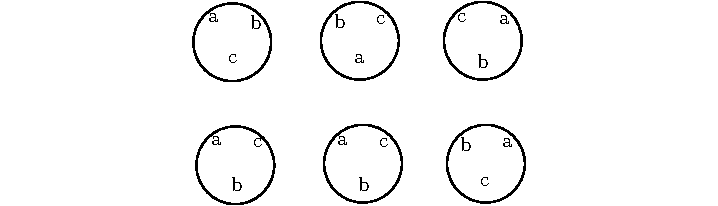
\includegraphics[width=0.9\linewidth]{Livro_files/figure-latex/figPermutacaoCircular-1} 

}

\caption{Permutação circular de três elementos.}\label{fig:figPermutacaoCircular}
\end{figure}

\begin{solution}
\iffalse{} {Solução. } \fi{}Consideramos os casais \(C_i\), para \(i=1,\ldots, n\) e definimos os \(n\) conjuntos a seguir
\(A_i =\) ``conjunto das permutações circulares das \(2n\) pessoas mas quais os membros do \(i\)-ésimo casal estejam juntos, para \(i=1,\ldots, n\)''.
Estamos procurando o complementar da união destes \(n\) conjuntos.
Veja que \(|A_i| = 2(2n-1)!\), pois o casal \(P_1,P_2\) pode se sentar de duas maneiras, a saber, \(P_1 P_2\) e \(P_2 P_1\), e, como estarão juntos na mesa circular, podem ser considerados como sendo uma única pessoa, sendo então \(n-1\) elementos no círculo.
Seguindo este mesmo raciocínio,
\begin{align}
|A_i \cap A_j| &= 2 \cdot 2 (2n - 2 -1)!, \\
|A_i \cap A_j \cap A_k| &= 2 \cdot 2 \cdot 2 (2n - 3 -1)!, \\
&\vdots \\
|A_i \cap A_j \cap \cdots \cap A_n| &= 2^n (2n - n -1)!.
\end{align}

Então,
\[\overline{A_i \cup A_j \cup \cdots \cup A_n} = (2n-1)! + \sum_{i=1}^{n}{n\choose i}(-1)^i2^i(2n-1-i)!.\]
\end{solution}

\hypertarget{a-funuxe7uxe3o-phi-de-euler}{%
\section{\texorpdfstring{A função \(\phi\) de Euler}{A função \textbackslash{}phi de Euler}}\label{a-funuxe7uxe3o-phi-de-euler}}

\begin{definition}
\protect\hypertarget{def:defPhiEuler}{}{\label{def:defPhiEuler} }Chamamos de função \(\phi\) de Euler a função que atribui a cada inteiro positivo \(m\) o número de inteiros menors do que ou iguais a \(m\) e relativamente primos com \(m\).
\end{definition}

\begin{theorem}
\protect\hypertarget{thm:teoValorPhi}{}{\label{thm:teoValorPhi} }O valor de \(\phi(m)\) é dado por
\[\phi(m) = m\bigg(1 - \frac{1}{p_1}\bigg)\bigg(1 - \frac{1}{p_2}\bigg)\cdots\bigg(1 - \frac{1}{p_r}\bigg),\]
em que \(p_1, p_2, \ldots, p_r\) são os divisores primos de \(m\), isto é, os primos na decomposição de \(m\) em fatores primos:
\[m = p_1^{\alpha_1}p_2^{\alpha_2}\cdots p_r^{\alpha_r}.\]
\end{theorem}

\begin{proof}
\iffalse{} {Prova. } \fi{}Como o valor de \(\phi(m)\) é o número de elementos no complementar da união dos \(A_i\)´s em \(A\), temos

\begin{align}
\phi (m) &= \Big| \overline{\bigcup_{i=1}^{r} A_i} \Big| \\
         &= \Big| \bigcap_{i=1}^{r} \overline{A_i} \Big| \\
         &= \Big| \Omega \setminus \bigcup_{i=1}^{r} A_i \Big| \\
         &= |A| - |A_1 \cup A_2 \cup \cdots \cup A_r| \\
         &= |A| - \sum_{i=1}^{r}|A_i| + \sum_{1\leq i<j}|A_i \cap A_j| + \cdots + (-1)^r|A_1\cap A_2\cap\cdots\cap A_r|.
\end{align}

Como
\begin{align} 
|A| &= m, &\quad |A_i| &= \bigg\lfloor{\frac{m}{p_i}}\bigg\rfloor, &\quad \\
|A_i \cap A_j| &= \bigg\lfloor{\frac{m}{p_i p_j}}\bigg\rfloor, &\quad 
|A_i \cap A_j \cap A_k| &= \bigg\lfloor{\frac{m}{p_i p_j p_k}}\bigg\rfloor,
\end{align}
\begin{align} 
&\vdots \\ |A_1 \cap A_2 \cap\cdots\cap A_r| &= \bigg\lfloor{\frac{m}{p_1 p_2 \cdots p_r}}\bigg\rfloor,
\end{align}

temos

\begin{align}
\phi(m) &= m - \sum_{i=1}^{r}\frac{m}{p_i} + \sum_{1\leq i<j}\frac{m}{p_i p_j} + \cdots + (-1)^r\frac{m}{p_1 p_2 \cdots p_r}\\
&= m \Big(1 - \sum_{i=1}^{r}\frac{1}{p_i} + \sum_{1\leq i<j}\frac{1}{p_i p_j} + \cdots + (-1)^r\frac{1}{p_1 p_2 \cdots p_r} \Big) \\
&= m \Big(1 - \frac{1}{p_1}\Big)\Big(1 - \frac{1}{p_2}\Big)\cdots\Big(1 - \frac{1}{p_r}\Big)
\end{align}
\end{proof}
{RELEMBRAR COMO ESSE ULTIMO PASSO É FEITO}

\begin{example}
\protect\hypertarget{exm:unnamed-chunk-76}{}{\label{exm:unnamed-chunk-76} }Calcular \(\phi(m)\) para \(m=2100\)
\end{example}

\begin{solution}
\iffalse{} {Solução. } \fi{}Como \(m=2^2\cdot 3\cdot 5\cdot 7\), temos
\[\phi(m) = 2100 \Big(1 - \frac{1}{2}\Big)\Big(1 - \frac{1}{3}\Big) \Big(1 - \frac{1}{5}\Big)\Big(1 - \frac{1}{7}\Big) = 2100 \frac{1}{2}\frac{2}{3}\frac{4}{5}\frac{6}{7} = 480.\]
\end{solution}

\begin{remark}
\iffalse{} {Observação. } \fi{}Se \(p=m\), com \(p\) primo, então \(\phi(p)=p-1.\)
\end{remark}

\hypertarget{mais-exemplos-com-permutauxe7uxf5es}{%
\section{Mais exemplos com permutações}\label{mais-exemplos-com-permutauxe7uxf5es}}

\begin{example}
\protect\hypertarget{exm:unnamed-chunk-79}{}{\label{exm:unnamed-chunk-79} }Determine o número de permutações simples dos elementos \(a_1, a_2, \ldots, a_n\) nas quais \(a_1\) está em primeiro ou \(a_2\) está em segundo lugar.
\end{example}

\begin{solution}
\iffalse{} {Solução. } \fi{}Seja \(A_1\) o conjunto das permutações em que \(a_1\) está em primeiro lugar e \(A_2\) o conjunto das permutações em que \(a_2\) está em segundo lugar.
É claro que \(|A_1|=|A_2|=(n-1)!\) e \(|A_1 \cap A_2| = (n-2)!\).
Logo, o número que procuramos é \(|A_\cup A_2|\),

\begin{align}
|A_\cup A_2| &= |A_1| + |A_2| - |A_1 \cap A_2| \\
&= (n-1)! + (n-1)! - (n-2)!\\
&= 2(n-1)! - (n-2)!\\
&= 2(n-1)(n-2)! - (n-2)!\\
&= (2n - 2-1)(n-2)!\\
&= (2n-3)(n-2)!.\\
\end{align}
\end{solution}

\begin{definition}[Permutação Caótica]
\protect\hypertarget{def:defPermCaotica}{}{\label{def:defPermCaotica} \iffalse (Permutação Caótica) \fi{} }Uma permutação de \(a_1, a_2, \ldots, a_n\) é chamada de caótica quanto nenhum dos \(a_i\)´s se encontra na posição original, isto é, na \(i\)-ésima posição.
\end{definition}

Seja \(A_i=\) ``o conjunto das permutações de \(a_1, a_2, \ldots, a_n\) tendo \(a_i\) no \(i\)-ésimo lugar''.
Para calcular o número de permutações caóticas, denotado por \(D_n\) (desarranjo), devems calcular o número de elementos que não pertencem a nenhum dos \(A_i\)´s:

\[D_n = \Bigg|\overline{\bigcup_{i=1}^{n} A_i} \Bigg| = \Bigg|{\bigcap_{i=1}^{n} \overline{A_i}}\Bigg|.\]

Veja que
\begin{align}
|A_i| &= (n-1)! &\qquad \text{existem $n$ termos iguais a esse na soma}\\
|A_i\cap A_j| &= (n-2)! &\qquad \text{existem $C_n^1$ termos iguais a esse na soma}\\
|A_i\cap A_j \cap A_k| &= (n-3)! &\qquad \text{existem $C_n^2$ termos iguais a esse na soma}\\
&\vdots \\
|A_1\cap\cdots\cap A_n| &= 1 &\qquad \text{existem $C_n^n$ termos iguais a esse na soma}.\\
\end{align}
Então,

\begin{align}
D_n = \Bigg|{\bigcap_{i=1}^{n} \overline{A_i}}\Bigg| 
&= n! - n(n-1)! + C_n^2(n-2)! - C_n^3(n-3)! + \cdots + (-1)^n\cdot 1 \\
&= n! - \frac{n!}{1} +  \frac{n!}{2!(n-2)!} - \frac{n!}{3!(n-3)!} + \cdots + (-1)^n\frac{n!}{n!}\\
&= n! \Bigg(1 - \frac{1}{1!} + \frac{1}{2!} - \frac{1}{3!} + \cdots +(-1)^n\frac{1}{n!}\Bigg).
\end{align}

\begin{example}
\protect\hypertarget{exm:unnamed-chunk-81}{}{\label{exm:unnamed-chunk-81} }Quantas permutações dos inteiros \(1,2,3,\ldots,10\) tem exatamente \(4\) dos números em suas posições originais?
\end{example}

\begin{solution}
\iffalse{} {Solução. } \fi{}Como não são fixados os \(4\) números que permanecerão nas suas posições originais, devemos escolher esstes números.
Essa escolha pode ser feita de \(C_{10}^4\) maneiras distintas.
Em seguinda, devemos permutar os \(6\) números restantes caoticamente.
Então, a resposta será
\[C_{10}^4 D_6 = \frac{10!}{4!6!} 6! \Bigg(1 - \frac{1}{1!} + \frac{1}{2!} - \frac{1}{3!} + \frac{1}{4!} - \frac{1}{5!} + \frac{1}{6!}\Bigg) = 55650.\]
\end{solution}

\hypertarget{contando-o-nuxfamero-de-funuxe7uxf5es}{%
\subsection{Contando o número de funções}\label{contando-o-nuxfamero-de-funuxe7uxf5es}}

\begin{theorem}
\protect\hypertarget{thm:teoFuncoesBijetoras}{}{\label{thm:teoFuncoesBijetoras} }Sejam \(A\) e \(B\) conjuntos, em que \(|A|=n\) e \(|B|=k\).
Se \(k=n\), \(n>0\), então o número de funções bijetoras \(f:A\rightarrow B\) é \(k!\).
\end{theorem}

\begin{proof}
\iffalse{} {Prova. } \fi{}Se em \(A\) existem \(n\) pontos \(a_1, \ldots, a_n\), temos \(n\) possíveis imagens para \(a_1\), \(n-1\) possíveis imagens para \(a_2\), \(n-2\) para \(a_3\), \(\ldots\), 1 para \(a_n\).
\end{proof}

\begin{theorem}
\protect\hypertarget{thm:teoFuncoesInjetoras}{}{\label{thm:teoFuncoesInjetoras} }Sejam \(A\) e \(B\) conjuntos, em que \(|A|=n\) e \(|B|=k\).
Se \(n\leq k\), então o número de funções injetoras \(f:A\rightarrow B\) é \(k(k-1)(k-3)\cdots(k-n-1)!\).
\end{theorem}

\begin{proof}
\iffalse{} {Prova. } \fi{}Exercício!
\end{proof}

\begin{proposition}
\protect\hypertarget{prp:unnamed-chunk-85}{}{\label{prp:unnamed-chunk-85} }Se \(|A|=m\) e \(|B|=n\), então o número de funções \(f:A\rightarrow B\) é \(n^m\)
\end{proposition}

\begin{proof}
\iffalse{} {Prova. } \fi{}(por indução)
Para \(m=0\), tempos que \(|A|=0\) e a única função é a função vazia.
Neste caso, \(n^0=1\).
Suponha que vale para \(m\) e assuma \(|A|=m+1\).
Seja \(a \in A\) (qualquer) e seja \(|A^\prime|=A\setminus\{a\}\), um conjunto tal que \(|A^\prime|=m\).
Qualquer função \(f:A\rightarrow B\) atribui um elemento \(f(a)\in B\) para \(a\) e \(f|_{A^\prime}\) sendo uma função de \(A^\prime\) à \(B\).
Pela hipótese de indução, existem \(n^m\) funções de \(A^\prime\) à \(B\).
Logo, existem \(n\) maneiras de atribuir \(f(a)\in B\) para \(a \in B\), logo, pelo Princípio Multiplicativo, existem
\[n\cdot n^m = n^{m+1}\]
funções de \(A\) à \(B\).
\end{proof}

Na contagem do número de apliciações sobrejetoras é que necessitamos do princípio de inclusão e exclusão.

\begin{theorem}
\protect\hypertarget{thm:teoFuncoesSobrejetoras}{}{\label{thm:teoFuncoesSobrejetoras} }Sejam \(A\) e \(B\) conjuntos, em que \(|A|=n\) e \(|B|=k\).
Para \(n\geq k\), o número de funções sobrejetoras \(f:A\rightarrow B\) é dado por
\[T(n,k) = \sum_{i=0}^{k}(-1)^i{k \choose i}(k-i)^n.\]
\end{theorem}

\begin{proof}
\iffalse{} {Prova. } \fi{}Como sabemos, uma função sobrejetora é tal que, para todo \(b \in B\), existe pelo menos um \(a \in A\) tal que \(f(a)=b\).
Como existem \(k^n\) funções de \(A\) em \(B\), vamos subtrair desse total o número de funções que não são sobrejetoras.

Considerando os elementos de \(B\), \(b_1, \ldots, b_k\), definimos \(C_i=\) ``conjunto de todas as funções \(f:A\rightarrow B\) tais que \(f^{-1}(b_i)=\emptyset\)'', isto é,
\(f(a)\neq b_i, \forall a \in A\).
Como uma função deixa de ser sobrejetora quanto pertence a pelo menos um dos \(C_i\)´s, para \(i=1,2,\ldots, k\), o conjunto de todas as funções não-sobrejetoras é
\[C_1 \cup C_2 \cup\cdots \cup C_k = \bigcup_{i=1}^{k}C_i.\]
Logo, pelo Princípio da Inclusão e Exclusão,
\[\Big|\bigcup_{i=1}^{k}C_i\Big| = \sum_{i=1}^{k}|C_i| - \sum_{1\leq i<j}^{}|C_i\cap C_j| + \sum_{1\leq i<j<l}^{}|C_i\cap C_j\cap C_l| + \cdots |C_i\cap\cdots\cap C_k|\]

Como \(|C_i|=(k-1)^n\), \(|C_i\cap C_j| = (k-2)^n, \ldots, |C_1\cap\ldots\cap C_k|=(k-k)^n\), temos
\begin{align}
  \Big|\bigcup_{i=1}^{k}C_i\Big| 
  &={k \choose 1}(k-1)^n - {k \choose 2}(k-2)^n + {k \choose 3}(k-3)^n + \cdots + {k \choose k}(k-k)^n \\
  &=\sum_{i=1}^{k}(-1)^{i-1}{k \choose i}(k-i)^n.
\end{align}

Subtraindo este número do total \(k^n\), temos

\[k^n-\sum_{i=1}^{k}(-1)^{i-1}{k \choose i}(k-i)^n = \sum_{i=0}^{k}(-1)^{i}{k \choose i}(k-i)^n.\]
\end{proof}

\begin{remark}
\iffalse{} {Observação. } \fi{}\(T(n,k)\) é o número de maneiras de se distirbuir \(n\) bolas distintas em \(k\) caixas distintas sem que nenhuma fique vazia.
\end{remark}

\begin{example}
\protect\hypertarget{exm:unnamed-chunk-89}{}{\label{exm:unnamed-chunk-89} }Consideremos um conjunto de \(9\) pessoas, sendo que todas sabem dirigir.
De quantas maneiras estas \(9\) pessoas podem se agrupar para levar \(4\) carros de Campinas à São Paulo?
\end{example}

\begin{solution}
\iffalse{} {Solução. } \fi{}Como todo carro deve ter um motorista, este número será igual ao núumero de funções sobrejetoras de um conjunto de \(9\) elementos num conjunto de \(4\) elementos.
Pelo Teorema \ref{thm:teoFuncoesSobrejetoras},

\begin{align}
T(9,4) &= \sum_{i=0}^{4}(-1)^k{4 \choose i}(4-i)^9 \\
&= {4 \choose 4} 4^9 - {4 \choose 1} 3^9 + {4 \choose 2} 2^9- {4 \choose 3} 1^9\\
&= 186480.
\end{align}
\end{solution}

\hypertarget{sem4}{%
\chapter{Semana 4}\label{sem4}}

\hypertarget{probabilidade}{%
\section{Probabilidade}\label{probabilidade}}

\begin{definition}[Espaço amostral]
\protect\hypertarget{def:defEspAmostral}{}{\label{def:defEspAmostral} \iffalse (Espaço amostral) \fi{} }O espaço amostral de um experimento é o conjunto de todos os resultados possíveis deste experimento.
Notação: \(\mathcal{S}.\)
\end{definition}

\begin{example}
\protect\hypertarget{exm:exCorrida}{}{\label{exm:exCorrida} }Defina o espaço amostral do seguinte experimento: ordem de chegada de uma corrida entre \(7\) pessoas numeradas de \(1\) a \(7\).
\end{example}

\begin{solution}
\iffalse{} {Solução. } \fi{}\(\mathcal{S}=\{\text{todas as $7!$ permutações de $\{1,2,3,4,5,6,7\}$}\}.\)
\end{solution}

\begin{example}
\protect\hypertarget{exm:exDuasMoedas}{}{\label{exm:exDuasMoedas} }Defina o espaço amostral do seguinte experimento: resultado do lançamento de duas moedas.
\end{example}

\begin{solution}
\iffalse{} {Solução. } \fi{}O espaço amostral é formado pelos quatro elementos a seguir
\[\mathcal{S}=\{(H,H),(H,T),(T,H),(T,T)\}.\]
O resultado será \((H,T)\) se a primeira moeda der \(cara\) e a segunda \(coroa\).
\end{solution}

\begin{definition}[Evento]
\protect\hypertarget{def:defEvento}{}{\label{def:defEvento} \iffalse (Evento) \fi{} }Qualquer subconjunto \(E\) do espaço amostral é conhecido como evento.
\end{definition}

Em outras palavras, um evento é um conjunto formado pelos possíveis resultados do experimento.
Se o resultado do experimento estiver contido em \(E\), dizemos que \(E\) ocorreu.

No Exemplo \ref{exm:exCorrida}, considere \(E=\{\text{todos os resultados em $\mathcal{S}$ começando com $3$}\}\), então \(E\) é o evento em que a pessoa identificada pelo número \(3\) vence a corrida.
Já no Exemplo \ref{exm:exDuasMoedas}, se \(E=\{(H,H),(H,T)\}\), então \(E\) é o evento em que a primeira moeda lançada dá \(cara\).

Para quaisquer dois eventos \(E\) e \(F\) de um espaço amostral \(\mathcal{S}\), definimos o novo evento \(E\cup F\) como sendo formado por todos os resultados que pertecem a \(E\) ou a \(F\) ou a \(E\) e \$F simultaneamente.
Isto é, o evento \(E\cup F\) ocorrerá se \(E\) ou \(F\) ocorrer.

\begin{example}
\protect\hypertarget{exm:unnamed-chunk-93}{}{\label{exm:unnamed-chunk-93} }No Exemplo \ref{exm:exDuasMoedas}, se \(E=\{(H,H),(H,T)\}\) é o evento em que dá \(cara\) no primeiro lançamento e \(F=\{(T,H)\}\), então
\(E\cup F=\{(H,H),(H,T),(T,H)\}\).
Assim, \(E\cup F\) ocorreria se desse \(cara\) em qualquer uma das duas moedas.
\end{example}

Para quaisquer dois eventos \(E\) e \(F\) de um espaço amostral \(\mathcal{S}\), definimos o evento \(EF\) (ou \(E\cap F\)), chamado de interseção entre \(E\) e \(F\), como sendo formado por todos os resultados que estão tanto em \(E\) quanto em \$F.

\begin{example}
\protect\hypertarget{exm:unnamed-chunk-94}{}{\label{exm:unnamed-chunk-94} }No Exemplo \ref{exm:exDuasMoedas}, se \(E=\{(H,H),(H,T),(T,H)\}\) é o evento em que pelo menos uma \(cara\) aparece nas duas moedas e \(F=\{(H,T),(T,H),(T,T)\}\) é o evento em que pelo menos uma coroa aparece, então
\[E\cap F=\{(H,T),(T,H)\}\]
é o evento em que exatamente uma \(cara\) e uma \(coroa\) aparecem.
\end{example}

Se \(EF=\emptyset\), então dizemos que \(E\) e \(F\) são mutualmente exclusivos.

\hypertarget{axiomas-de-probabilidade}{%
\section{Axiomas de Probabilidade}\label{axiomas-de-probabilidade}}

Uma maneira de definir a probabilidade de um evento é em termos de sua frequência relativa: suponhamos que um experimento, cujo espaço amostral é \(\mathcal{S}\), seja realizado repetidamente em condições exatamente iguais.
Para cada evento \(E \subseteq \mathcal{S}\), definimos \(n(E)\) como o número de vezes que \(E\) ocorre nas \(n\) primeiras repetições do experimento.
Então \(P(E)\), a probabilidade do evento \(E\), é definida como
\[P(E) = \lim_{n \rightarrow \infty} \frac{n(E)}{n}.\]

Há um inconveniente nesta definição: como saberemos que \(\frac{n(E)}{n}\) convergirá para algum valor limite constante que será o mesmo para cada possível sequência de repetições do experimento?

Vamos considerar a abordagem axiomática moderna da teoria da probabilidade.
Então, vamos assumir que, para cada evento \(E \subseteq \mathcal{S}\), existe um valor \(P(E)\) chamado de probabilidade de ocorrência do evento \(E\).
Vamos supor então que todas as probabilidade satisfazem certo conjunto de axiomas.

Considere um experimento cujo espaço amostral é \(\mathcal{S}\).
Para cada evento \(E\) de \(\mathcal{S}\), assumimos que o número \(P(E)\) seja definido e satisfaça os três axiomas a seguir.

\begin{itemize}
\tightlist
\item
  Axioma 1: \(0 \leq P(E) leq 1\);
\item
  Axioma 2: \(P(S) = 1\);
\item
  Axioma 3: para cada sequencia de eventos mutualmente exclusivos \(E_1, E_2, \ldots\) (ou seja, \(E_i E_j=\emptyset\) quando \(i\neq j\)), \(P\big(\cup_{i=1}^{\infty}E_i\big)=\sum_{i=1}^{\infty}E_i\).
\end{itemize}

Se considerarmos a sequeência de eventos \(E_1, E_2, \ldots\), em que \(E_1=\mathcal{S}\) e \(E_i=\emptyset\) para \(i>1\), então, como os eventos são mutualmente exclusivos e \(\mathcal{S}=\cup_{i=1}^{\infty}E_i\), teremos, pelo Axioma 3,
\[P(\mathcal{S})=\sum_{i=1}^{\infty}P(E_i) = P(\mathcal{S}) + \sum_{i=}^{\infty}P(E_i),\]
o que implica que \(P(\emptyset)=0\).
Isto é, o evento vazio tem probabilidade nula.
Daí seque que, para qualquer sequência de eventos mutualmente exclusivos \(E_1, E_2, \ldots, E_n\),
\[P\Bigg(\bigcup_{i=1}^{\infty}E_i\Bigg) = \sum_{i=}^{n}P(E_i).\]

\begin{example}
\protect\hypertarget{exm:unnamed-chunk-95}{}{\label{exm:unnamed-chunk-95} }Se um dado é lançado e supormos que seus seis lados tenham a mesma probabilidade de aparecer, então teremos \(P(\{1\})=\) \(P(\{2\})=\) \(P(\{3\})=\) \(P(\{4\})=\) \(P(\{5\})=\) \(P(\{6\})=\) \(\frac{1}{6}\).
Do Axioma 3, temos que a probabilidade de sair um número par é igual a
\[P(\{2,4,6\}) = P(\{ 2 \})+P(\{ 4 \})+P(\{ 6 \}) = \frac{3}{6} = \frac{1}{2}.\]
\end{example}

\begin{proposition}
\protect\hypertarget{prp:propComplementar}{}{\label{prp:propComplementar} }\[P(E^c) = 1 - P(E^c).\]
\end{proposition}

Em palavras, a Proposição \ref{prp:propComplementar} afirma que a probabilidade de um evento não ocorrer é igual à 1 menos a probabilidade dele ocorrer.

\begin{proof}
\iffalse{} {Prova. } \fi{}Note que \(E\) e \(E^c\) são sempre mutualmente exclusivos e, como \(E\cup E^c=\mathcal{S}\), temos, pelos Axiomas 2 e 3,
\[1 = P(\mathcal{S}) = P(E\cup E^c) = P(E) + P(E^c)\]
\end{proof}

\begin{proposition}
\protect\hypertarget{prp:propProbSubConjunto}{}{\label{prp:propProbSubConjunto} }Se \(E \subset F\), então \(P(E) \leq P(F)\).
\end{proposition}

\begin{proof}
\iffalse{} {Prova. } \fi{}Como \(E \subset F\), podemos expressar \(F\) como \(F = E \cup E^c F\).
Portanto, como \(E\) e \(E^c F\) são mutualmente exclusivos, obtemos, pelo Axioma 3,
\[P(F) = P(E) + P(E^c F),\]
o que prova o resultado, já que \(P( E^c F)\geq 0\).
\end{proof}

\begin{proposition}
\protect\hypertarget{prp:propProbUniao}{}{\label{prp:propProbUniao} }\[P(E \cup F) = P(E) \leq P(F) - P(E\cap F).\]
\end{proposition}

\begin{proof}
\iffalse{} {Prova. } \fi{}Note que \(E \cup F = E \cup E^c F\).
Do Axioma 3 obtemos
\[P(E \cup F) = P(E \cup E^c F) = P(E) + P(E^c F).\]
Além disso, como \(F = EF\cup E^c F\), obtemos do Axioma 3
\[P(F) = P(EF) + P(E^c F),\]
ou, equivalentemente, \(P(E^c F) = P(F) - P(EF)\), o que completa a demonstração.
\end{proof}

\begin{example}
\protect\hypertarget{exm:unnamed-chunk-99}{}{\label{exm:unnamed-chunk-99} }Uma pessoa leva dois livros para ler durante as férias.
A probabilidaide dela gostar do primeiro livro é \(0{,}5\), de gostar do segundo livro é \(0{,}4\) e de gostar de ambos os livros é \(0{,}3\).
Qual a probabilidade de que essa pessoa não goste de nenhum dos livros?
\end{example}

\begin{solution}
\iffalse{} {Solução. } \fi{}Seja \(L_i\) o evento ``a pessoa gosta do livro \(i\)'', \(i=1,2\).
Então, a probabilidade dessa pessoa gostar de pelo menos um livro é
\[P(L_1 \cap L_2) = P(L_1) + P(L_2) - P(L_1L_2) = 0{,}5+0{,}4-0{,}3=0{,}6.\]

Como o evento ``a pessoa não gosta de nenhum dos livros'' é o complementar do evento em que ela gosta de pelo menos um deles, obtemos como resultado
\[P\big(L_1^c \cap L_2^c\big) = P\big((L_1^c \cup L_2)^c\big) = 1 - P\big(L_1^c \cup L_2\big) = 0{,}4.\]
\end{solution}

\begin{proposition}
\protect\hypertarget{prp:propInclusaoExclusao}{}{\label{prp:propInclusaoExclusao} }\begin{align}
P(E_1\cup E_2 \cup\cdots\cup E_n) = \sum_{i=1}^{n}P(E_i) &- \sum_{1\leq i <j}P(E_i E_j) \\
&+ \cdots (-1)^{r+1}\sum_{1\leq i <j<\cdots<r}^{}P(E_i E_j \cdots E_r) +\cdots  \\
&+(-1)^{n+1}P(E_1 E_2 \cdots E_n).
\end{align}
\end{proposition}

\begin{remark}
\iffalse{} {Observação. } \fi{}A soma \(\sum_{1\leq i <j<\cdots<r}^{}P(E_i E_j \cdots E_r)\) é feita ao longo de todos os \({n \choose r}\) subconjuntos possíveis de tamanho \(r\) do conjunto \(\{1,2,3,\ldots, n\}.\)
\end{remark}

\begin{proof}
\iffalse{} {Prova. } \fi{}Exercício!
Dica: semelhante ao visto no Princípio de Inclusão e Exclusão (veja o Teorema \ref{thm:teoPrincInclExcl}).
\end{proof}

\hypertarget{espauxe7os-amostrais-com-resultados-igualmente-provuxe1veis}{%
\section{Espaços amostrais com resultados igualmente prováveis}\label{espauxe7os-amostrais-com-resultados-igualmente-provuxe1veis}}

Em muitos experimentos é natural supor que todos os resultados presentes no espaço amostral sejam igualmente prováveis.
Por exemplo, considere um experimento cujo espaço amostral \(\mathcal{S}\) é um conjunto finito, digamos \(\mathcal{S}=\{1,2,\ldots, n\}\).
Se supormos que
\[P(\{1\})= P(\{2\})= \cdots = P(\{n\})= \frac{1}{6},\]
então, pelos Axiomas 2 e 3, temos que (por quê?)
\[P(\{i\})=\frac{1}{n}, \qquad i=1,2,\ldots, n.\]
A partir da expressão acima e do Axioma 3, temos que, para cada evento \(E\),

\[P(E)=\frac{\text{número de resultados em }E}{\text{número de resultados em } \mathcal{S}}.\]

\begin{example}
\protect\hypertarget{exm:unnamed-chunk-103}{}{\label{exm:unnamed-chunk-103} }Se dois dados são lançados, qual é a probabilidade de que a soma das daces de cima seja igual a \(7\)?
\end{example}

\begin{solution}
\iffalse{} {Solução. } \fi{}Assumindo que os \(36\) resultados possíveis são equiprováveis, como há \(6\) resultados possíveis que resultam na soma dos dados se \(7\) -- isto é, \((1,6), (2,5), (3,4), (4,3), (5,2), (6,1)\) -- a probabilidade desejada é igual a \(\frac{6}{36}=\frac{1}{6}.\)
\end{solution}

\begin{example}
\protect\hypertarget{exm:unnamed-chunk-105}{}{\label{exm:unnamed-chunk-105} }Se três bolas são retiradas aleatoriamente de um recipiente contendo \(6\) bolas brancas e \(5\) bolas pretas, qual é a probabilidade de que uma das bolas seja branca e as outras duas sejam pretas?
\end{example}

\begin{solution}
\iffalse{} {Solução. } \fi{}Se considerarmos a ordem de seleção das bolas como sendo relevante, então o espaço amostral é formado por \(11\cdot 10\cdot 9 = 990\) resultados.
Além disso, existem \(6\cdot 5\cdot 4 = 120\) resultados nos quais a primeira bola selecionada é branca e as outras duas são pretas; \(5\cdot g\cdot 4 = 120\) resultados \(5\cdot 4\cdot 6 = 120\) resultados nos quais as primeiras duas bolas são pretas e a terceira é branca.
Portanto, supondo que retiradas aleatoriamente signifique que cada evento do espaço amostral seja igualmente provável, vemos que a probabilidade desejada é
\[\frac{120 + 120 + 120}{990}=\frac{4}{11}.\]
\end{solution}

\begin{solution}
\iffalse{} {Solução. } \fi{}(alternativa)
Podemos considerar o resultado do experimento como sendo o conjunto desordenado de bolas retiradas.
Então, existem \({11 \choose 3}=165\) resultados no espaço amostral.
Nesse caso, cada conjunto de 3 bolas corresponde a \(3!\) resultados quando a ordem de seleção é levada em consideração.
Como consequência, se for considerado que todos resultados são equiprováveis quando a ordem da seleção é importante, tem-se que estes continuam equiprováveis quando o resultado considerado é um conjunto desordenado de bolas selecionadas.
Dessa forma, usando esta última representação do experimentos, vemos que a probabilidade desejada é
\[\frac{{6\choose 1}{5\choose 2}}{{11\choose 3}} = \frac{4}{11}.\]
\end{solution}

\begin{example}
\protect\hypertarget{exm:unnamed-chunk-108}{}{\label{exm:unnamed-chunk-108} }Um comitê de 5 pessoas deve ser selecionado de um grupo de 6 homens e 9 mulheres.
Se a seleção for feita aleatoriamente, qua é a probabilidade de que o comitê seja formado por 3 homens e 2 mulheres?
\end{example}

\begin{solution}
\iffalse{} {Solução. } \fi{}\[\frac{{6\choose 3}{9 \choose 2}}{{15 \choose 5}} = \frac{240}{1001}.\]
\end{solution}

\begin{example}
\protect\hypertarget{exm:unnamed-chunk-110}{}{\label{exm:unnamed-chunk-110} }Suponha que \(n+m\) bolas, das quais \(n\) são vermelhas e \(m\) são azuis, sejam arranjadas em uma sequência linear de forma que todas as \((m+n)!\) sequências possíveis sejam igualmente prováveis.
Se gravarmos o resultado deste experimento lsitando apenas as cores das bolas sucessivas, mostre que todos os resultados possíveis permanecem igualmente prováveis.
\end{example}

\begin{solution}
\iffalse{} {Solução. } \fi{}Considere qualquer uma das \((m+n)!\) sequências possíveis e note que qualquer permutação das bolas vermelhas entre si e das bolas azuis entre si não muda a sequência de cores.
Como resultado, cada sequência de cores tem probabilidade de ocorrência igual a \(\frac{n!m!}{(n+m)!}.\)
Por exemplo, suponha que há 2 bolas vermelhas nomeadas \(v_1\) e \(v_2\) e duas bolas azuis, nomeadas \(a_1\) e \(a_2\).
Então, das \(4!\) possíveis sequências, \(2!2!\) delas resultarão em qualquer combinação de cores especificada.
Por exemplo, as ordenações a seguir resulta na alternância de cores em bolas adjacentes, com uma bola vermelha na frente
\begin{align}
v_1 a_1 v_2 a_2, & \qquad v_1 a_2 v_2 a_1, \\
v_2 a_1 v_1 a_2, & \qquad v_2 a_2 v_1 a_1.
\end{align}
Portanto, cada uma das possíveis sequências de cores tem probabilidade \(\frac{4}{24}=\frac{1}{6}\) de ocorrer.
\end{solution}

\begin{example}
\protect\hypertarget{exm:unnamed-chunk-112}{}{\label{exm:unnamed-chunk-112} }Se \(n\) pessoas se encontram no interior de uma sala, qual é a probabilide de que duas pessoas não celebrem o aniversário no mesmo dia do ano?
Quão grande precisa ser \(n\) para que essa probabilidade seja menor que \(0{,}5\).
\end{example}

\begin{solution}
\iffalse{} {Solução. } \fi{}Como cada pessoa pode celebrar seu aniversário em qualquer um dos 365 dias do ano, há um total de \(365^n\) resultados possíveis (estamos considerando apenas anos não bisextos!).
Supondo que cada resultado seja igualmente provável, vemos que a probabilidade desejada é igual a
\[\frac{365\cdot 364\cdot 363 \cdots (365-n+1)}{365^n}.\]

Quando \(n\geq 23\), esta probabilidade é menor que \(\frac{1}{2}\).
Isto é, 23 pessoas ou mais na sala, então a probabilidade de que pelo menos duas delas façam aniversário no mesmo dia é maior que \(\frac{1}{2}\).
\end{solution}

\begin{example}[Permutação caótica revisitada]
\protect\hypertarget{exm:unnamed-chunk-114}{}{\label{exm:unnamed-chunk-114} \iffalse (Permutação caótica revisitada) \fi{} }Suponha que cada uma das \(N\) pessoas presentes em uma festa junina atire seu chapeu para o centro de uma roda.
Os chapeus são misturadaos e então cada pessoa seleciona aleatoriamente um deles.
Qual é a probabilidade de que nenhuma das pessoas selecione o seu próprio chapeu?
\end{example}

\begin{solution}
\iffalse{} {Solução. } \fi{}Seja \(E_i, i=1,2,\ldots,N\), o evento em que a \(i\)-ésima pessoa seleciona seu próprio chapeu.
Pela Proposição \ref{prp:propInclusaoExclusao}, \(P(\cup_{i=1}^{N}E_i)\), a probabilidade de que pelo menos um dos presentes na festa selecione o seu próprio chapeu é dada por
\begin{align}
P(\cup_{i=1}^{N}E_i)=P(E_1\cup E_2 \cup\cdots\cup E_n) =& \sum_{i=1}^{N}P(E_i) - \sum_{1\leq i <j}P(E_i E_j) \\ &+ \cdots +(-1)^{n+1}P(E_1 E_2 \cdots E_N).
\end{align}

Se interpretarmos o resultado deste experimento como um vetor de \(N\) números, em que o \(i\)-ésimo elemento corresponde ao número do chapeu jogado pela \(i\)-ésima pessoa, então existem \(n!\) resultados possíveis.
Além disso, \(E_{i_1}E_{i_2}\cdots E_{i_n}\), o evento em que cada uma das \(n\) pessoas
\(i_1, i_2, \ldots, i_n\) seleciona o seu próprio chapeu pode ocorrer de qualquer uma das \((N-n)(N-n-1)\cdots 1=(N-n)!\) maneiras possíveis.
Assim, supondo que todos os \(N!\) resultados possíveis sejam igualmente prováveis, vemos que
\[P(E_{i_1}E_{i_2}\cdots E_{i_n}) = \frac{(N-n)!}{N!}.\]

Além disso, como existem \({N \choose n}\) termos em \(\sum_{1\leq i_1<i_2 < \cdots < i_n}P(E_{i_1}E_{i_2}\cdots E_{i_n})\), temos que
\[\sum_{1\leq i_1<i_2 < \cdots < i_n}P(E_{i_1}E_{i_2}\cdots E_{i_n}) = \frac{N!}{(N-n)!n!}\frac{(N-n)!}{N!} = \frac{1}{n!}.\]
Logo,
\[P\Bigg(\bigcup_{i=1}^{N}\Bigg) = 1 - \frac{1}{2!} + \frac{1}{3!} - \cdots + (-1)^{N+1}\frac{1}{N!}.\]
Portanto, a probabilidade de que nenhuma das pessoas selecione o seu próprio chapeu é
\begin{equation}
1 - P\Bigg(\bigcup_{i=1}^{N}\Bigg) = 1 - 1 + \frac{1}{2!} - \frac{1}{3!} + \cdots - (-1)^{N+1}\frac{1}{N!}
\label{eq:exemploChapeu}
\end{equation}
\end{solution}

\begin{remark}
\iffalse{} {Observação. } \fi{}Para \(n\) grande, a Expressão \eqref{eq:exemploChapeu} converge para \(\mathrm{e}^{-1}\approx 0{,}36788\).
\end{remark}

\hypertarget{sem5}{%
\chapter{Semana 5}\label{sem5}}

\hypertarget{probabilidade-condicional-e-independuxeancia}{%
\section{Probabilidade condicional e independência}\label{probabilidade-condicional-e-independuxeancia}}

Suponha que lancemos dois dados, cada um com 36 resultados possíveis é igualmente provável e portanto tem probabilidade \(\frac{1}{36}\).
Digamos que o primeiro dado seja um 3.
Então, dada essa informação, qual é a probabilidade de que a soma dos dois dado seja 8?

Sabendo que saiu um 3 no dado inicial, existirão no máximo 6 resultados possíveis para o nosso experimento, isto é, \((3,1) ,(3,2) ,(3,3) ,(3,4) ,(3,5) ,(3,6)\).
Como cada um desses resultados tinha originalmente a mesma probabilidade de ocorrência, os resultados deveriam continuar a ter probabilidades iguais.
Dado que o primeiro dado é 3, a probabilidade (condicional) de cada um dos resultados possíveis é \(\frac{1}{6}\), enquanto a probabilidade (condicional) dos outros 30 pontos no espaço amostral é zero.
Com isso, a probabilidade desejada será igual a \(\frac{1}{6}\).

\begin{definition}[Probabilidade Condicional]
\protect\hypertarget{def:defProbCond}{}{\label{def:defProbCond} \iffalse (Probabilidade Condicional) \fi{} }Sejam \(E\) e \(F\) dois eventos tais que \(P(F>0)\).
A probabilidade condicional de que \$E ocorra dado que \(F\) ocorreu é representada por
\begin{equation}
P(E|F) = \frac{P(EF)}{P(F)}.
\label{eq:condicional}
\end{equation}
\end{definition}

\begin{example}
\protect\hypertarget{exm:unnamed-chunk-117}{}{\label{exm:unnamed-chunk-117} }Uma moeda é lançada duas vezes.
Supondo que todos os quatro pontos no espaço amostral \(\mathcal{S} = \{(H,H), (H,T), (T,H), (T,T)\}\) sejam equiprováveis, qual a probabilidade condicional de que dê \(cara\) (\(H\)) em ambas as jogadas dado que (a) dê \(cara\) na primeira jogada? (b) dê \(cara\) em pelo menos uma das jogadas?
\end{example}

\begin{solution}
\iffalse{} {Solução. } \fi{}Sejam \(B=\{(H,H)\}\) o evento em que ambos lançamentos dão cara, \(F=\{(H,H),(H,T)\}\) o evento em que dá \(cara\) no primeiro lançamento e \(A=\{(H,H),(H,T),(T,H)\}\) o evento em que pelo menos uma \(cara\) ocorre.
Então, para o item (a) temos

\begin{align}
P(B|F) &= \frac{P(BF)}{P(F)}\\
&=\frac{P(\{(H,H)\})}{P(\{(H,H),(H,T)\})} &&\\
&=\frac{1/4}{2/4}=\frac{1}{2}.
\end{align}

E para o item (b)

\begin{align}
P(B|A) &= \frac{P(BA)}{P(A)}\\
&=\frac{P(\{(H,H)\})}{P(\{(H,H),(H,T),(T,H)\})} &&\\
&=\frac{1/4}{3/4}=\frac{1}{3}.
\end{align}
\end{solution}

Multiplicando ambos os lados da Expressão \eqref{eq:condicional} por \(P(F)\), obtemos
\begin{equation}
P(E|F)P(F) = P(EF).
\label{eq:condicional2}
\end{equation}

\begin{example}
\protect\hypertarget{exm:unnamed-chunk-119}{}{\label{exm:unnamed-chunk-119} }Marcela está indecisa quanto a fazer a disciplina de Análise Combinatória ou Introdução à Probabilidade.
Ela estima que sua probabilidade de conseguir um conceito \(A\) seria de \(\frac{2}{3}\) em Análise Combinatória e \(\frac{1}{2}\) em Introdução à Probabilidade.
Se Marcela decide basear sua escolha no lançamento de uma moeda honesta, qual é a probabilidade de que ela obtenha A em Análise Combinatória?
\end{example}

\begin{solution}
\iffalse{} {Solução. } \fi{}Suponha que \(C\) seja o evento em que Marcela faz o curso de Análise Combinatória e \(A\) o evento em que ela tira \(A\) independentemente do curso que fizer.
Então
\[P(CA) = P(C)P(A|C) = \frac{1}{2}\frac{2}{3} = \frac{1}{3}.\]
\end{solution}

\begin{example}
\protect\hypertarget{exm:unnamed-chunk-121}{}{\label{exm:unnamed-chunk-121} }Suponha que uma urna contenha 8 bolas vermelhas e 4 bolas brancas.
Retira-se duas bolas sem reposição.
(a) se supõe-se que em cada retirada cada bola na urna tenha a mesma probabilidade de ser escolhida, qual é a probabilidade de que ambas as bolas retiradas sejam vermelhas?
(b) Suponha que as bolas tenham tamanhos diferentes (vermelha tem peso \(r\) e a branca tem peso \(w\)) e que a probabilidade de que a próxima bola a ser retirada da urna seja igual ao peso da bola dividido pela soma dos pesos de todas as bolas na urna naquele momento.
Qual é a probabilidade de que ambas bolas sejam vermelhas?
\end{example}

\begin{solution}
\iffalse{} {Solução. } \fi{}Defina os eventos \(R_1 =\) ``primeira bola retirada é vermelha'' e \(R_2 =\) ``seg9unda bola retirada é vermelha''.
(a) Dado que a primeira bola é vermelha, existem 7 bolas vermelhas e 4 bolas brancas restantes, de forma que \(P(R_2|R_1) = 7/11\).
Como \(P(R_1)=8/12\), a probabilidade desejada é
\[P(R_1 R_2) = P(R_1)P(R_2|R_1) = \frac{2}{3}\frac{7}{11} = \frac{14}{33}.\]
Alternativamente, \(P(R_1 R_2) = {{8\choose 2}}/{{12\choose 2}}\).

Para o item (b) vamos usar \(P(R_1 R_2) = P(R_1)P(R_2 | R_1)\).
Numere as bolas vermelhas e suponha que \(B_i, i=1, \ldots, 8\) seja o evento em que a primeira bola retirada é uma bola vermelha de numero \(i\).
Então,
\[P(R_1) = P\Bigg(\bigcup_{i=1}^{8}B_i\Bigg) = \sum_{i=1}^{8}P(B_i) = 8\cdot \frac{r}{8r+4w}.\]

Se a primeira bola é vermelha, a urna passa a conter 7 bolas vermelhas e 4 bolas brancas.
Assim, pelo mesmo argumento acima,
\[P(R_2 | R_1) = 7\cdot \frac{r}{7r+4w}.\]
Portanto, a probabilidade desejada é
\[P(R_1 R_2) = \frac{8r}{8r+4w}\frac{7r}{7r+4w}.\]
\end{solution}

Uma generalização da Equação \eqref{eq:condicional2} fornece uma expressão para a probabilidade da interseção de um número arbitrário de eventos.

\begin{proposition}[Regra da multiplicação]
\protect\hypertarget{prp:unnamed-chunk-123}{}{\label{prp:unnamed-chunk-123} \iffalse (Regra da multiplicação) \fi{} }\begin{equation}
P(E_1 E_2 \cdots E_n) = P(E_1)P(E_2|E_1)P(E_3|E_1 E_2)\cdots P(E_n|E_1 E_2 \cdots E_{n-1}).
\label{eq:condicional3}
\end{equation}
\end{proposition}

\begin{proof}
\iffalse{} {Prova. } \fi{}Aplicando a Definição \ref{def:defProbCond} de probabilidade condicional ao lado direito da Equação \eqref{eq:condicional3}, temos
\[P(E_1) \frac{P(E_1E_2)}{P(E_1)} \frac{P(E_1 E_2 E_3)}{P(E_1 E_2)} \cdots \frac{P(E_1 E_2 \cdots E_n)}{P(E_1 E_2 \cdots E_{n-1})} = P(E_1 E_2 \cdots E_n).\]
\end{proof}

\hypertarget{fuxf3rmula-de-bayes}{%
\section{Fórmula de Bayes}\label{fuxf3rmula-de-bayes}}

Sejam os eventos \(E\) e \(F\).
Podemos expressar \(E\) como
\[E = EF \cup EF^c.\]
Note que \((EF) \cap (EF^c)=\emptyset\), assim, pelo Axioma 3,
\begin{align}
P(E) &= P(EF) + P(EF^c)\\
&= P(E|F)P(F) + P(E|F^c)P(F^c).
\label{eq:complementar}
\end{align}

ADICIONAR FIGURA INTUITIVA SOBRE ESSE RESULTADO.

A Equação \eqref{eq:complementar} diz que a probabilidade do evento \(E\) é uma média ponderada da probabilidade condicional de \(E\) dado que o evento \(F\) ocorreu e da probabilidade condicional de \(E\) dado que \(F\) não ocorreu.
Esta fórmula é útil porque seu uso muitas vezes nos permite determinar a probabilidad ed um evento com base na condição de ocorrência ou não de um segundo evento.

\begin{example}
\protect\hypertarget{exm:unnamed-chunk-125}{}{\label{exm:unnamed-chunk-125} }Uma companhia de seguros acredita que pessoas podem ser divididas em duas classes: aquelas que são propensas a acidentes e aquelas que não são.
A estatística da companhia mostra que uma pessoa propensa a acidadentes tem probabilidade de \(0{,}4\) de sofrer umacidente dentro de um período fixo de 1 ano, enquanto que essa probabilidade cai para \(0{,}2\) no caso de uma pessoa não propensa a acidentes.
Se supormos que \(30\%\) da população é propensa a acidentes, (a) qual é a probabilidade de que um novo segurado sofra um acidente no período de um ano posterior à compra de sua apólice?
(b) Suponha que um novo segurado sofra um acidente em menos de um ano após a compra da apólice.
Qual é a probabilidade de que ele seja propenso a acidentes?
\end{example}

\begin{solution}
\iffalse{} {Solução. } \fi{}Vamos definir o evento \(A_1\) como sendo o evento em que ``o segurado sofre um acidente no período de um ano após a compra de sua apólice'' e \(A\) como ``o segurado é propenso a acidentes''.
Assim, a probabilidade desejada no item (a) é
\begin{align}
P(A_1) &= P(A_1|A)P(A) + P(A_1|A^c)P(A^c)\\
&= 0{,}4\cdot 0{,}3 + 0{,}2\cdot 0{,}7 = 0{,}26.
\end{align}

Para o item (b), queremos obter \(P(A|A_1)\).
Então,

\[P(A|A_1) = \frac{P(A A_1)}{P(A_1)} = \frac{P(A_1|A)P(A)}{P(A_1)} = \frac{ 0{,}3\cdot 0{,}4}{ 0{,}26} = \frac{6}{13}.\]
\end{solution}

A Equação \eqref{eq:complementar} pode ser generalizada da seguinte maneira.
Suponha que \(F_1, F_2, \ldots, F_n\) sejam eventos mutualmente exclusivos tais que

\[\bigcup_{i=1}^{n}F_i=\mathcal{S}.\]
Escrevendo \[E = \bigcup_{i=1}^{n}EF_i,\]

e usando o fato de que os eventos \(EF_i, i=1,\ldots, n\) são mutualmentne exclusivos, obtemos

\begin{equation}
P(E) =  \sum_{i=1}^{n}P(EF_i) = \sum_{i=1}^{n}P(E|F_i)P(F_i).
\label{eq:particao}
\end{equation}

A Equação \eqref{eq:particao} mostra que, para dados eventos \(F_1, F_2, \ldots, F_n\), dos quais \textbf{um e apenas um} deve ocorrer, podemos calcular \(P(E)\) primeiro analizando as condições em que \(F_i\) ocorre.
Além disso, a Equação \eqref{eq:particao} diz que \(P(E)\) é ogial à mmédia ponderada de \(P(E|F_i)\), com cada termo sendo ponderado pela probabilidade do evento ao qual está condicionado.

Considerando a mesma sequência de eventos \(F_1, F_2, \ldots, F_n\), uma partição de \(\mathcal{S}\), suponha que \(E\) tenha ocorrido e que estejamos interessados em determinar qual dos \(F_j\) ocorreu.
Então pela generalização apresentada pela Equação \eqref{eq:particao}, temos a Proposição \ref{prp:bayes} a seguir.

\begin{proposition}[Fórmula de Bayes]
\protect\hypertarget{prp:bayes}{}{\label{prp:bayes} \iffalse (Fórmula de Bayes) \fi{} }\begin{align}
P(F_j|E) &= \frac{P(EF_j)}{P(E)}\\
&= \frac{P(E|F_j)P(F_j)}{\sum_{i=1}^{n}P(E|F_i)P(F_i)}.
\end{align}
\end{proposition}

\begin{example}
\protect\hypertarget{exm:unnamed-chunk-127}{}{\label{exm:unnamed-chunk-127} }Uma caixa contés 3 tipos de lâmpadas.
A probabilidade de que uma lâmpada do tipo 1 funcione por mais de 100h é igual a \(0{,}7\) e as probabilidades referentes às lâmpadas do tipoo 2 e 3 correspondem à \(0{,}4\) e \(0{,}3\), respectivamente.
Suponha que \(20\%\) das lâmpadas na caixa sejam do tipo 1, \(30\%\) sejam do tipo 2 e \(50\%\) do tipo 3.
(a) Qual a probabilidade de que uma lâmpada alteatoriamente escolhida funcione mais que 100 horas?
(b) Dado que uma lâmpada tenha durado mais de 100 horas, qual é a probabilidade de que ela seja uma lâmpada do tipo \(j, j=1,2,3\)?
\end{example}

\begin{solution}
\iffalse{} {Solução. } \fi{}Vamos definir \(A\) como o evento ``a lâmpada escolhida funciona mais do que 100h'' e \(F_j\) como ``a lâmpada do tipo \(j\) é escolhida'', para \(j=1,2,3\).
Então, para o item (a) temos
\begin{align}
P(A) & = \sum_{j=1}^{3}P(A|F_j)P(F_j)\\
& = P(A|F_1)P(F_1) + P(A|F_2)P(F_2) + P(A|F_3)P(F_3)\\
& = 0{,}7\cdot 0{,}2 + 0{,}4\cdot 0{,}3 + 0{,}3\cdot 0{,}5\\
&= 0{,}41.
\end{align}

Para o item (b), vamos usar a fórmula de Bayes (veja a Proposição \ref{prp:bayes})

\[P(F_j|A) = 
  \frac{P(AF_j)}{P(A)} = \frac{P(A|F_j)P(F_j)}{0{,}41}.\]

Assim,
\begin{align}
P(F_1|A) &= 
  \frac{0{,}7\cdot 0{,}2}{0{,}41} = \frac{11}{41} = 0{,}341, \\
P(F_j|A) &= 
  \frac{0{,}4\cdot 0{,}3}{0{,}41} = \frac{12}{41} = 0{,}293, \\
P(F_j|A) &= 
  \frac{0{,}3\cdot 0{,}5}{0{,}41} = \frac{15}{41} = 0{,}366.
\end{align}

Note que, enquanto a probabilidade de uma lâmpada do tipo 1 ser escolhida é de apenas \(0{,}2\), a informação de que a lanterna funcionou por mais de 100 horas aumenta a probabildiade do evento \(E_1\) para \(0{,}341\).
\end{solution}

\begin{definition}[Independência entre eventos]
\protect\hypertarget{def:defIndep}{}{\label{def:defIndep} \iffalse (Independência entre eventos) \fi{} }Dois eventos \(E\) e \(F\) são chamados de independentes se
\[P(EF) = P(E)P(F).\]
Notação: \(E\perp F\).
\end{definition}

\begin{example}
\protect\hypertarget{exm:unnamed-chunk-129}{}{\label{exm:unnamed-chunk-129} }Duas moedas são lançadas e supões-se que os 4 resultados possíveis são igualmente prováveis.
Se \(E\) é o evento em que a primeira moeda dá cara e \(F\) é o evento em que a segunda moeda dá corora, então pode-se dizer que \(E\) e \(F\) são independentes?
\end{example}

\begin{solution}
\iffalse{} {Solução. } \fi{}Sabemos que os 4 resultados possíveis deste experimento são \((h,h),(h,t),(t,h),(t,t)\), em que \(h\) representa cara e \(t\) representa coroa.
Então, vamos verificar se existe independência entre \(E\) e \(F\) através da Definição \ref{def:defIndep}.
\begin{align}
P(EF) &= P(\{(h,t)\}) = \frac{1}{4},\\
P(E) &= P(\{(h,h),(h,t)\}) = \frac{1}{2},\\
P(F) &= P(\{(h,t),(t,t)\}) = \frac{1}{2}.\\
\end{align}

Portanto, vemos que \(P(EF) = P(E)P(F)\), e \(E \perp F\).
\end{solution}

\begin{proposition}
\protect\hypertarget{prp:unnamed-chunk-131}{}{\label{prp:unnamed-chunk-131} }Se \(E\) e \(F\) são independentes, então \(E\perp F^c\).
\end{proposition}

\begin{proof}
\iffalse{} {Prova. } \fi{}Suponha que \(E\) e \(F\) são independentes.
Como \(E=EF\cup EF^c\) e \((EF)\cap (EF^c)=\emptyset\), temos

\begin{align}
P(E) &= P(EF) + P(EF^c)\\
&=P(E)P(F) + P(EF^c).
\end{align}

Equivalentemente,
\begin{align}
P(EF^c) &= P(E) - P(E)P(F)\\
&=P(E)\big[1-P(F)\big].\\
&=P(E)P(F^c).
\end{align}
\end{proof}

\hypertarget{variuxe1veis-aleatuxf3rias}{%
\section{Variáveis Aleatórias}\label{variuxe1veis-aleatuxf3rias}}

Ao realizar um experimento, frequentemente estamos interessados principalmente em alguma função do resultado e não do resultado em si.
Essas grandezas de interesse, ou essas funções reais definidas no espaço amostral, são conhecidas como \textbf{variáveis aleatórias}.
Como o valor da variável aleatória é determinado pelo resultado do experimento, podemos atribuir probabilidades à estes possíveis valores.

\begin{example}
\protect\hypertarget{exm:unnamed-chunk-133}{}{\label{exm:unnamed-chunk-133} }Considere o experimento de lançar 3 moedas honestas.
Se \(Y\) representar o número de \(caras\) que apareceram, então \(Y\) é uma variável aleatória que pode assumir um dos valores \(0,1,2\) ou \(3\) com probabilidades
\begin{align}
P(Y=0) &= P(\{(t,t,t)\}) = \frac{1}{8}, \\
P(Y=1) &= P(\{(t,t,h),(t,h,t),(h,t,t)\}) = \frac{3}{8}, \\
P(Y=2) &= P(\{(t,h,h),(h,t,h),(h,h,t)\}) = \frac{3}{8}, \\
P(Y=3) &= P(\{(h,h,h)\}) = \frac{1}{8}.
\end{align}
\end{example}

\begin{example}
\protect\hypertarget{exm:unnamed-chunk-134}{}{\label{exm:unnamed-chunk-134} }Três bolas são selecionadas aleatoriamente e sem reposição de uma urna contendo 20 bolas numeradas de 1 a 20.
Se apostarmos que pelo menos uma das bolas selecionadas tem um número maior ou igual a 17, qual é a probabilidade de vencermos a aposta?
\end{example}

\begin{solution}
\iffalse{} {Solução. } \fi{}Seja \(X\) o maior número selecionado.
Então \(X\) é uma variável aleatória que pode ter qualquer um dos valores \(3, 4, \ldots, 20\).
Se supormos que cada uma das \({20\choose 3}\) seleções possíveis tem a mesma probabilidade de ocorrer, então
\(P(X=i) = {{i-1} \choose 2}/{20\choose 3}, i = 3, 4, \ldots, 20.\)\$

Temos, então, que
\(P(X \geq 17)=\) \(P(X=17) +\) \(P(X=18) +\) \(P(X=19) +\) \(P(X=20) =\) \(0{,}509.\)
\end{solution}

\begin{definition}[Função de distribuição acumulada]
\protect\hypertarget{def:defFDA}{}{\label{def:defFDA} \iffalse (Função de distribuição acumulada) \fi{} }Para uma variável aleatórioa \(X\), a funçãp \(F\) definida por
\[F(x) = P(X\leq x), \qquad -\infty<x<\infty\]
é chamada de função de distribuição acumulada, ou, mais simplismente, de função de distribuição de \(X\).
\end{definition}

\begin{remark}
\iffalse{} {Observação. } \fi{}Se \(a \leq b\), então \(\{X\leq a\} \subseteq \{X \leq b\}\), logo \(F(a)\leq F(b)\).
Note que \(F(x)\) é uma função não-decrescente.
\end{remark}

\begin{definition}[Variável discreta]
\protect\hypertarget{def:defVAdiscreta}{}{\label{def:defVAdiscreta} \iffalse (Variável discreta) \fi{} }Uma variável aleatória que pode assumir no máximo um número contável de valores possíveis é chamada de variável aleatória discreta.
\end{definition}

Para uma variável aleatória discreta \(X\), definimos a função discreta de probabilidade (ou função de probabilidade) \(p(a)\) de \(X\) como
\[p(a) = P(\{X=a\}).\]
A função \(p(a)\) é positiva para no máxima um número contável de valores de \(a\).
Isto é, se \(X\) deve assumir um dos valoreos \(x_1, x_2, \ldots\), então
\begin{align}
p(x_i) \geq 0, &\quad \text{para } i=1,2,\ldots \\
p(x_i) = 0, &\quad \text{para todos os demais valores de $x$.}
\end{align}

Como \(X\) deve receber um dos valores \(X_i\), temos
\[\sum_{i=1}^{\infty}p(x_i)=1.\]
A função de distirbuição acumulada \(F\) pode ser expressa em termos de \(p(a)\) como
\[F(a) = \sum_{x \leq a}p(x).\]

\begin{example}
\protect\hypertarget{exm:unnamed-chunk-137}{}{\label{exm:unnamed-chunk-137} }Se \(X\) tem uma função de probabilidade dada por
\[p(1) = \frac{1}{4}, \quad p(2) = \frac{1}{2}, \quad p(3) = \frac{1}{8}, \quad p(4) = \frac{1}{8},\]
então, sua função de distribuição acumulada é

\begin{equation}
  F(a) =
    \begin{cases}
      0 & \text{se } a < 1\\
      1/4 & \text{se } 1 \leq a < 2\\
      3/4 & \text{se } 2 \leq a < 3\\
      7/8 & \text{se } 3 \leq a < 4\\
      1 & \text{se } 4 \leq a\\
    \end{cases}       
\end{equation}

\begin{verbatim}
  INSERIR FIGURA DA PAGINA 7 DO ARQUIVO DA SEMANA 5
\end{verbatim}
\end{example}

\hypertarget{sem6}{%
\chapter{Semana 6}\label{sem6}}

\begin{definition}[Valore esperado]
\protect\hypertarget{def:defEsperanca}{}{\label{def:defEsperanca} \iffalse (Valore esperado) \fi{} }Se \(X\) é uma variável aleatória com função de probabilidade \(p(x)\), então o valor esperado, ou esperança, de \(X\) é definido por
\[E(X) = \sum_{x:p(x)>0} x\cdot p(x).\]
\end{definition}

Note que \(E(X)\) é uma média ponderada dos possíveis valores que \(X\) pode assumir, com cada valor sendo ponderado pela probabilidade de que \(X\) seja igual a esse valor.

\begin{example}
\protect\hypertarget{exm:esperancaDado}{}{\label{exm:esperancaDado} }Determine \(E(X)\), em que \(X\) é o resultado obtido ao lançar um dado honesto.
\end{example}

\begin{solution}
\iffalse{} {Solução. } \fi{}Como \(p(1)=\) \(p(2)=\) \(p(3)=\) \(p(4)=\) \(p(5)=\) \(p(6)=\) \(1/6\), temos

\[E(X) = 1\cdot \frac{1}{6} +2\cdot \frac{1}{6}+3\cdot \frac{1}{6}+4\cdot \frac{1}{6}+5\cdot \frac{1}{6}+6\cdot \frac{1}{6}=\frac{7}{2}.\]
\end{solution}

\begin{example}
\protect\hypertarget{exm:unnamed-chunk-139}{}{\label{exm:unnamed-chunk-139} }Dizemos que \(I\) é uma variável indicadora do evento \(A\) se
\begin{equation}
  F(a) =
    \begin{cases}
      1 & \text{se $A$ ocorre,}\\
      0 & \text{se $A^c$ ocorre.}
    \end{cases}       
\end{equation}
Determine \(E(X).\)
\end{example}

\begin{solution}
\iffalse{} {Solução. } \fi{}Como \(p(1)=P(A)\) e \(p(0)=P(A^c)\), temos
\[E(I)=1\cdot P(A) + 0\cdot (1-P(A)) = P(A.)\]
Assim, o valor esperado da variável indicadora do evento \(A\) é igual à probabilidade de ocorrência de \(A\).
\end{solution}

\hypertarget{esperanuxe7a-de-uma-funuxe7uxe3o-de-uma-variuxe1vel-aleatuxf3ria}{%
\section{Esperança de uma função de uma variável aleatória}\label{esperanuxe7a-de-uma-funuxe7uxe3o-de-uma-variuxe1vel-aleatuxf3ria}}

Seja \(X\) uma variável aleatória discreta e suponha que queriamos calcular o valor esperado de alguma função de \(X\), digamos \(g(X)\).
Como \(g(x)\) é uma variável aleatória discreta, ela tem função de probabilidade que pode ser deerminada a partir da função de probabilidade de \(X\), assim, podemos calcular \(E[g(x)]\) usando a Definição \ref{def:defEsperanca}.

\begin{example}
\protect\hypertarget{exm:exX2}{}{\label{exm:exX2} }Seja \(X\) uma variável aleatória que pode receber os valores \(-1, 0, 1\) com probabilidades \(P(X=-1)=0{,}2\), \(P(X=0)=0{,}5\) e \(P(X=1)=0{,}3\).
Calcule \(E(X^2)\).
\end{example}

\begin{solution}
\iffalse{} {Solução. } \fi{}Seja \(Y=X^2\), então a função de probabilidade de \(Y\) é dada por
\begin{align}
P(Y=1) &= P(X=-1) + P(X=1) = 0{,}5,\\ 
P(Y=0) &= P(X=0) = 0{,}5.\\ 
\end{align}
Logo,
\[E(X^2) = E(Y) = 1\cdot 0{,}5 + 0\cdot 0{,}5 = 0{,}5.\]
Observe que \(0{,}5 = E(X^2) \neq [E(X)]^2 = 0{,}01\).
\end{solution}

\begin{proposition}
\protect\hypertarget{prp:propGx}{}{\label{prp:propGx} }Se \(X\) é uma variável aleatória discreta que pode receber os valores \(x_i, i\geq 1\), com respectivas probabilidade \(p(x_i)\), então, para qualquer função real \(g\)
\[E[g(x)] = \sum_i g(x_i)p(x_i).\]
\end{proposition}

\begin{proof}
\iffalse{} {Prova. } \fi{}Vamos agrupar todos os termos em \(\sum_i g(x_i)p(x_i)\) com mesmo valor de \(g(x_i)\).
Especificamente, suponha que \(y_j, j\geq 1\), represente os diferentes valores de \(g(x_i), i\geq 1\).
Então, o agrupamento de todos os \(g(x_i)\) com valores iguais resulta em
\begin{align}
\sum_i g(x_i)p(x_i) &= \sum_j \sum_{i:g(x_i)=y_j} g(x_i)\cdot p(x_i)\\
&=\sum_j \sum_{i:g(x_i)=y_j} y_j\cdot p(x_i)\\
&=\sum_j y_j \sum_{i:g(x_i)=y_j} p(x_i)\\
&=\sum_j y_j \cdot P(g(X)=y_i)\\
&= E(g(X)).
\end{align}
\end{proof}

\begin{example}
\protect\hypertarget{exm:unnamed-chunk-143}{}{\label{exm:unnamed-chunk-143} }No Exemplo \ref{exm:exX2}, podemos calcular \(E(X^2)\) de uma forma mais direta, usando o resultado da Proposição \ref{prp:propGx}.
\begin{align}
E(X^2) &= (-1)^2\cdot 0{,}2 + 0^2\cdot 0{,}5 + 1^2\cdot 0{,}3\\
&= 1\cdot(0{,}2+0{,}3) + 0\cdot 0{,}5\\
&= 0{,}5.
\end{align}
\end{example}

\begin{corollary}
\protect\hypertarget{cor:corEsperanca}{}{\label{cor:corEsperanca} }Se \(a\) e \(b\) são constantes, então \[E(aX+b) = aE(X)+b.\]
\end{corollary}

\begin{proof}
\iffalse{} {Prova. } \fi{}\begin{align}
E(aX+b) &= \sum_{x:p(x)>0}(ax+b)\cdot p(x)\\
&=a\sum_{x:p(x)>0}x \cdot p(x) + b\sum_{x:p(x)>0}p(x)\\
&= aE(X) + b.
\end{align}
\end{proof}

\begin{definition}[Variância]
\protect\hypertarget{def:unnamed-chunk-145}{}{\label{def:unnamed-chunk-145} \iffalse (Variância) \fi{} }Se \(X\) é uma variável aleatória com média \(\mu\), então a variância de \(X\), representada por \(\mathrm{Var}(X)\) é definida como
\[\mathrm{Var}(X) = E\big[(X-\mu)^2\big].\]
\end{definition}

Uma fórmula alternativa para o cálculo de \(\mathrm{Var}(X)\) é deduzida a seguir.

\begin{align}
\mathrm{Var}(X) &= E\big[(X-\mu)^2\big] \\
&= \sum_x (x-\mu)^2p(x) \\
&= \sum_x (x^2 - 2\mu x + \mu^2)p(x)\\
&= \sum_x x^2p(x) - 2\mu\sum_x xp(x) + \mu^2\sum_x p(x)\\
&= E(X^2) - 2\mu^2 + \mu^2\\
&= E(X^2) - \mu^2.
\end{align}

Assim,
\[\mathrm{Var}(X) = E\big(X^2\big)-\big[E(X)\big]^2.\]
Na prática, essa é uma maneira mais fácil de calcular \(\mathrm{Var}(X)\).

\begin{example}
\protect\hypertarget{exm:unnamed-chunk-146}{}{\label{exm:unnamed-chunk-146} }calcule \(\mathrm{Var}(X)\) se \(X\) representa o resultado do lançamento de um dado honesto.
\end{example}

\begin{solution}
\iffalse{} {Solução. } \fi{}Vimos no Exemplo \ref{exm:esperancaDado} que \(E(X) =\frac{7}{2}\).
Note que
\[E(X^2) = 1^2\cdot \frac{1}{6} +2^2\cdot \frac{1}{6}+3^2\cdot \frac{1}{6}+4^2\cdot \frac{1}{6}+5^2\cdot \frac{1}{6}+6^2\cdot \frac{1}{6}=91\cdot\frac{1}{6}.\]
Com isso,
\[\mathrm{Var}(X) = \frac{91}{6} - \bigg(\frac{7}{2}\bigg) = \frac{35}{12}.\]
\end{solution}

\begin{corollary}
\protect\hypertarget{cor:unnamed-chunk-148}{}{\label{cor:unnamed-chunk-148} }Para \(a\) e \(b\) constantes, \[\mathrm{Var}(aX+b) = a^2\mathrm{Var}(X).\]
\end{corollary}

\begin{proof}
\iffalse{} {Prova. } \fi{}Considere \(\mu=E(X)\) e lembre-se que \(E(aX+b)=aE(X)+b\) (veja Corolário \ref{cor:corEsperanca}).
Portanto,
\begin{align}
\mathrm{Var}(aX+b) &= E\bigg[\big((aX+b)-(a\mu+b)\big)^2\bigg] \\
&= E\bigg[\big((aX+b-a\mu-b)\big)^2\bigg] \\
&= E\big[a^2(X-\mu)^2\big] \\
&= a^2 E\big[(X-\mu)^2\big] \\
&= a^2 \mathrm{Var}(X).
\end{align}
\end{proof}

\begin{definition}[Desvio Padrão]
\protect\hypertarget{def:unnamed-chunk-150}{}{\label{def:unnamed-chunk-150} \iffalse (Desvio Padrão) \fi{} }A quantidade \(\sqrt{\mathrm{Var}(X)}\) é chamada de desvio padrão de \(X\).
\[\mathrm{SD}(X) = \sqrt{\mathrm{Var}(X)}.\]
\end{definition}

\hypertarget{variuxe1veis-aleatuxf3rias-discretas}{%
\section{Variáveis Aleatórias Discretas}\label{variuxe1veis-aleatuxf3rias-discretas}}

Suponha que um experimento cujo resultado possa ser classificado como sucesso ou fracasso seja realizado.
Se \(X=1\) quando o resultado é sucesso e \(X=0\) quando fracasso, então, a função de probabilidade de \(X\) é dada por
\begin{align}
p(0) &= P(\{X=0\}) = 1-p,\\
p(1) &= P(\{X=1\}) = p,
\label{eq:bernoulli}
\end{align}
em que \(p\), \(0\leq p \leq 1\), é a probabilidade de que a tentativa seja um sucesso.
Uma variável aleatória \(X\) é chamada de \textbf{variável aleatória de Bernoulli} se sua função de probabilidade for dada como na Expressão \eqref{eq:bernoulli}, para \(p \in (0,1)\).
Notação: \(X \sim \mathrm{Bernoulli}(p)\).

Suponha agora que \(n\) tentativas independentes, cada uma com probabilidade \(p\) de sucesso e probabilidade de fracasso \(1-p\), sejam realizadas.
Se \(Y\) representa o número de sucessos que ocorrem nas \(n\) tentativas, enão \(Y\) é uma \textbf{variável aleatória binomial} com parâmetros \((n,p)\).
Note que uma variável aleatória Bernoulli é uma variável aleatória binomial com parâmetros \((1,p)\).
Notação: \(X \sim \mathrm{bin}(n,p)\).

A função de probabilidade de uma variável aleatória binomial com parâmetros \((n,p)\) é
\[p(i) = {n \choose i}p^i(1-p^n-1{}),\]
para \(i=0,1,2,\ldots,n\).

Pelo teorema binomial (CADE A REFERENCIA?), a soma das probabilidades é igual a \(1\)
\[\sum_{i=0}^{\infty} = \sum_{i=0}^{n}{n \choose i}p^i(1-p)^{n-1} = [p+(1-p)]^n=1.\]

\begin{example}
\protect\hypertarget{exm:unnamed-chunk-151}{}{\label{exm:unnamed-chunk-151} }Cinco moedas honeas são lançadas.
Se os resultados por hipótese são independentes, determine a função de probabilidade do número de caras obtido.
\end{example}

\begin{solution}
\iffalse{} {Solução. } \fi{}Se \(X\) é o número de caras (sucessos) obtidas, então \(X\sim \mathrm{bin}(n=5p=1/2)\).
Então
\begin{align}
P(X=0) &= {5 \choose 0} \bigg(\frac{1}{2}\bigg)^0 \bigg(\frac{1}{2}\bigg)^5 = \frac{1}{32},\\
P(X=1) &= {5 \choose 1} \bigg(\frac{1}{2}\bigg)^1 \bigg(\frac{1}{2}\bigg)^4 = \frac{5}{32},\\
P(X=2) &= {5 \choose 2} \bigg(\frac{1}{2}\bigg)^2 \bigg(\frac{1}{2}\bigg)^3 = \frac{10}{32},\\
P(X=3) &= {5 \choose 3} \bigg(\frac{1}{2}\bigg)^3 \bigg(\frac{1}{2}\bigg)^2 = \frac{10}{32},\\
P(X=4) &= {5 \choose 4} \bigg(\frac{1}{2}\bigg)^4 \bigg(\frac{1}{2}\bigg)^1 = \frac{5}{32},\\
P(X=5) &= {5 \choose 5} \bigg(\frac{1}{2}\bigg)^5 \bigg(\frac{1}{2}\bigg)^0 = \frac{1}{32}.
\end{align}
\end{solution}

\begin{example}
\protect\hypertarget{exm:unnamed-chunk-153}{}{\label{exm:unnamed-chunk-153} }Os parafusos produzidos em certa empresa tem probabilidade \(0{,}01\) de apresentar defeitos, independentemente uns dos outros.
A empresa vende os parafusos em pacotes com \(10\) unidades e oferece uma garantia se mais de 1 parafuso apresentar defeito.
Que proporção de pacotes vendidos a emprese deve trocar?
\end{example}

\begin{solution}
\iffalse{} {Solução. } \fi{}Defina \(X=\) ``número de parafusos defeituosos em um pacote''.
Note que \(X \sim \mathrm{bin}(10, 0{,}01)\).
Então, temos que calcular
\begin{align}
P(X > 1) &= 1 - \big[P(X=0)+P(X=1)\big] \\
&= 1 - P(X=0)-P(X=1)\\
&= 1 - {10 \choose 0}(0{,}01)^0(0{,}99)^10-{10 \choose 1}(0{,}01)^1(0{,}99)^9\\
&= 0{,}004.
\end{align}
\end{solution}

\hypertarget{funuxe7uxf5es-conjuntamente-distribuuxeddas}{%
\section{Funções conjuntamente distribuídas}\label{funuxe7uxf5es-conjuntamente-distribuuxeddas}}

Frequentemente estamos interessados em analisar a probabilidade de duas ou mais variáveis aleatórias simultaneamente.
Definimos a função discreta de probabilidade conjunta de \(X\) e \(Y\) como
\[p(x,y) = P(X=x, Y=y).\]
A função de probabilidade de \(X\) pode ser obtida de de \(p(x,y)\) por
\[p_X(x) = P(X=x) = \sum_{y:p(x,y)>0}p(x,y),\]
similarmente
\[p_Y(x) = P(Y=y) = \sum_{x:p(x,y)>0}p(x,y).\]

\begin{proposition}
\protect\hypertarget{prp:unnamed-chunk-155}{}{\label{prp:unnamed-chunk-155} }Se \(X\) e \(Y\) tem função de probabilidade conjunta \(p(x,y)\), então
\end{proposition}
\[E\big[g(X,Y)\big] = \sum_{x}\sum_{y}g(x,y)p(x,y).\]

Suponha que \(E(X)\) e \(E(Y)\) sejam finitas e faça \(g(X,Y)=X+Y\).
Então,
\begin{align}
E[X+Y] &= \sum_{x}\sum_{y}(x+y)p(x,y)\\
&=\sum_{x}\sum_{y}x p(x,y) + \sum_{x}\sum_{y}y p(x,y)\\
&=\sum_{x}x\sum_{y} p(x,y) + \sum_{y}y\sum_{y} p(x,y)\\
&=\sum_{x}x p(x) + \sum_{y}y p(y)\\
&= E(X) + E(Y).
\label{eq:esperancaSoma}
\end{align}

\begin{proposition}
\protect\hypertarget{prp:propSomaVar}{}{\label{prp:propSomaVar} }Se \(X\) e \(Y\) são variáveis aleatórias independentes, então
\[\mathrm{Var}(X+Y)=\mathrm{Var}(X)+\mathrm{Var}(Y).\]
\end{proposition}

\begin{example}
\protect\hypertarget{exm:unnamed-chunk-156}{}{\label{exm:unnamed-chunk-156} }Suponha que 3 bolas brancas seja sorteadas de uma urna contendo 3 bolas vermelhas, 4 bolas brancas e 5 bolas azuis.
Se \(X\) e \(Y\) representam, respectivamaenten, o número de bolas vermelhas e brancas escolhidas, determine a função de probabilidade conjunta de \(X\) e \(Y\).
\end{example}
\begin{solution}
\iffalse{} {Solução. } \fi{}A função de probabilidade conjunta de \(X\) e \(Y\), \(p(i,j)=P(X=i,Y=j)\) é dada por
\begin{align}
p(0,0) &= \frac{{3\choose 0}{4\choose 0}{5\choose 3}}{{12 \choose 3}}, 
  &\qquad p(1,0) &= \frac{{3\choose 1}{4\choose 0}{5\choose 2}}{{12 \choose 3}},\\
p(0,1) &= \frac{{3\choose 0}{4\choose 1}{5\choose 2}}{{12 \choose 3}}, 
  &\qquad p(1,1) &= \frac{{3\choose 1}{4\choose 1}{5\choose 1}}{{12 \choose 3}},\\
p(0,2) &= \frac{{3\choose 0}{4\choose 2}{5\choose 2}}{{12 \choose 3}}, 
  &\qquad p(1,2) &= \frac{{3\choose 1}{4\choose 2}{5\choose 0}}{{12 \choose 3}},\\
p(0,3) &= \frac{{3\choose 0}{4\choose 3}{5\choose 0}}{{12 \choose 3}},
  &\qquad p(1,3) &= 0,\\
p(2,0) &= \frac{{3\choose 2}{4\choose 0}{5\choose 1}}{{12 \choose 3}}, 
  &\qquad p(2,1) &= \frac{{3\choose 2}{4\choose 1}{5\choose 0}}{{12 \choose 3}},\\
p(3,0) &= \frac{{3\choose 3}{4\choose 0}{5\choose 0}}{{12 \choose 3}}. 
\end{align}

Estas probabilidades pode ser apresentadas em forma de tabela ADICIONAR TABELA AQUI.
\end{solution}

\hypertarget{propriedades-das-variuxe1veis-aleatuxf3rias-binomiais}{%
\section{Propriedades das variáveis aleatórias binomiais}\label{propriedades-das-variuxe1veis-aleatuxf3rias-binomiais}}

Seja \(X\sim\mathrm{Bernoulli}(p)\).
Então, \[E(X) = 0\cdot P(X=0)+1\cdot P(X=1)=0\cdot (1-p) + 1\cdot p = p.\]
E, para calcular \(\mathrm{Var}(X)\), temos que obter
\[E(X^2)=0^2\cdot P(X=0)+1^2\cdot P(X=1)= p.\]
Então, \(\mathrm{Var}(X)=p - p^2=p(1-p).\)

Agora, \(sejam X_1, X_2, \cdots X_n\) variáveis aleatórias independentes entre si tais que \(X_i \sim\mathrm{Bernoulli}(p), i=1,\ldots n.\)
Vamos definir \(Y = \sum_{i=1}^{n}X_i =\) \(X_1 + \cdots + X_n.\)
Então \(Y\sim\mathrm{bin}(n,p)\) (por quê?), e, pela seguindo um raciocínio similar ao apresentado na Expressão \eqref{eq:esperancaSoma},
\[E[Y] = E\bigg[ \sum_{i=1}^{n}X_i \bigg] = \sum_{i=1}^{n}E[X_i]=n p.\]
E, pela Proposição \ref{prp:propSomaVar},
\[\mathrm{Var}(Y) = \mathrm{Var}\bigg(\sum_{i=1}^{n}X_i \bigg)=\sum_{i=1}^{n}\mathrm{Var}(X)=np(1-p).\]

\bibliography{book.bib,packages.bib}

\end{document}
